\documentclass[]{book}
\usepackage{lmodern}
\usepackage{amssymb,amsmath}
\usepackage{ifxetex,ifluatex}
\usepackage{fixltx2e} % provides \textsubscript
\ifnum 0\ifxetex 1\fi\ifluatex 1\fi=0 % if pdftex
  \usepackage[T1]{fontenc}
  \usepackage[utf8]{inputenc}
  \usepackage{eurosym}
\else % if luatex or xelatex
  \ifxetex
    \usepackage{mathspec}
  \else
    \usepackage{fontspec}
  \fi
  \defaultfontfeatures{Ligatures=TeX,Scale=MatchLowercase}
  \newcommand{\euro}{€}
\fi
% use upquote if available, for straight quotes in verbatim environments
\IfFileExists{upquote.sty}{\usepackage{upquote}}{}
% use microtype if available
\IfFileExists{microtype.sty}{%
\usepackage{microtype}
\UseMicrotypeSet[protrusion]{basicmath} % disable protrusion for tt fonts
}{}
\usepackage[margin=1in]{geometry}
\usepackage{hyperref}
\hypersetup{unicode=true,
            pdftitle={Economic and legals aspects of EMS - Support notes},
            pdfauthor={Técnico Lisboa},
            pdfborder={0 0 0},
            breaklinks=true}
\urlstyle{same}  % don't use monospace font for urls
\usepackage{natbib}
\bibliographystyle{apalike}
\usepackage{longtable,booktabs}
\usepackage{graphicx,grffile}
\makeatletter
\def\maxwidth{\ifdim\Gin@nat@width>\linewidth\linewidth\else\Gin@nat@width\fi}
\def\maxheight{\ifdim\Gin@nat@height>\textheight\textheight\else\Gin@nat@height\fi}
\makeatother
% Scale images if necessary, so that they will not overflow the page
% margins by default, and it is still possible to overwrite the defaults
% using explicit options in \includegraphics[width, height, ...]{}
\setkeys{Gin}{width=\maxwidth,height=\maxheight,keepaspectratio}
\IfFileExists{parskip.sty}{%
\usepackage{parskip}
}{% else
\setlength{\parindent}{0pt}
\setlength{\parskip}{6pt plus 2pt minus 1pt}
}
\setlength{\emergencystretch}{3em}  % prevent overfull lines
\providecommand{\tightlist}{%
  \setlength{\itemsep}{0pt}\setlength{\parskip}{0pt}}
\setcounter{secnumdepth}{5}
% Redefines (sub)paragraphs to behave more like sections
\ifx\paragraph\undefined\else
\let\oldparagraph\paragraph
\renewcommand{\paragraph}[1]{\oldparagraph{#1}\mbox{}}
\fi
\ifx\subparagraph\undefined\else
\let\oldsubparagraph\subparagraph
\renewcommand{\subparagraph}[1]{\oldsubparagraph{#1}\mbox{}}
\fi

%%% Use protect on footnotes to avoid problems with footnotes in titles
\let\rmarkdownfootnote\footnote%
\def\footnote{\protect\rmarkdownfootnote}

%%% Change title format to be more compact
\usepackage{titling}

% Create subtitle command for use in maketitle
\newcommand{\subtitle}[1]{
  \posttitle{
    \begin{center}\large#1\end{center}
    }
}

\setlength{\droptitle}{-2em}
  \title{Economic and legals aspects of EMS - Support notes}
  \pretitle{\vspace{\droptitle}\centering\huge}
  \posttitle{\par}
  \author{Técnico Lisboa}
  \preauthor{\centering\large\emph}
  \postauthor{\par}
  \predate{\centering\large\emph}
  \postdate{\par}
  \date{2018-02-04}

\usepackage{booktabs}
\usepackage{amsthm}
\makeatletter
\def\thm@space@setup{%
  \thm@preskip=8pt plus 2pt minus 4pt
  \thm@postskip=\thm@preskip
}
\makeatother

\usepackage{amsthm}
\newtheorem{theorem}{Theorem}[chapter]
\newtheorem{lemma}{Lemma}[chapter]
\theoremstyle{definition}
\newtheorem{definition}{Definition}[chapter]
\newtheorem{corollary}{Corollary}[chapter]
\newtheorem{proposition}{Proposition}[chapter]
\theoremstyle{definition}
\newtheorem{example}{Example}[chapter]
\theoremstyle{definition}
\newtheorem{exercise}{Exercise}[chapter]
\theoremstyle{remark}
\newtheorem*{remark}{Remark}
\newtheorem*{solution}{Solution}
\begin{document}
\maketitle

{
\setcounter{tocdepth}{1}
\tableofcontents
}
\chapter{Abstract}\label{abstract}

Chaters

\chapter{Scope, Limits and Methodology}\label{Scope}

\section{Scope and Limits}\label{scope-and-limits}

\section{Methodology}\label{methodology}

\chapter{Energy Prices}\label{energy-prices}

\section{Market design}\label{market-design}

Currently we are at a market design shift, where some countries are
already under liberalized market, others in transition.

Most Utilities operated under a Monopoly, namely a horizontal one, where
Generation, Transmission, Distribution and Delivery, was done by the
same entity.

\begin{figure}[htbp]
\centering
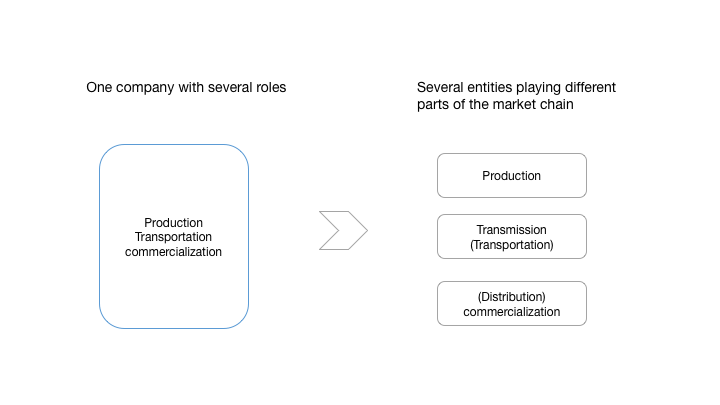
\includegraphics[width=1.00000\textwidth]{/Users/dvf/desktop/eba gitbook/Images/image12.png}
\caption{}
\end{figure}

To get to a fully to liberalized market, Europe has chosen an ownership
unbundling model, where infrastructure access plays a central role.

Regulation of the infrastructure access´ prices, or guarantee a fair
access to infrastructure so as the need to guarantee safety so as
sustainability of supply, are central issues when arguing about a fully
integrated Energy Market.

The split of generation, transportation (and grid operations \&
management) and commercialization, is reshaping the energy sector. The
consolidation and integration of the EU Energy Market presents a great
opportunity for several stakeholders and a challenge to consolidated
utilities companies.

When dealing with industries that have a common infrastructure, as
utilities (which includes energy and water), telecoms, access to
infrastructure plays a central role. You can just think of activities
where building infrastructure by each player would be undoable, so they
all share the same. Most, namely in Europe, were build by Governments,
where access do energy, water, telecommunications was a competence of
Governments.

So when liberalizing markets, Antitrust and competition are central
concerns on creating and promoting a fair and competitive market. The
ownership unbundling model (regulation of the infrastructure access´
prices) is one models used where:

Infrastructure´s assets belongs to the state (even if concession may be
considered for long periods of time, under public interest).

There is the coexistence of Free market and last resort suppliers, so
the need to regulate relationships between liberalized market and last
resort supplier so as these two with the end consumers.

The Pricing (of using the grid), such as : historical cost, incremental
costs, Retail Minus, Free access, Price Caps -- will promote different
incentives, will define the behavior of the company managing the grip.
For example, if you put a price cap and don´t pay any contribution for
maintenance and improvement of the overall grid, most likely you will
have and overexploitation of the grid. On the other hand, if you have
any top limit for investment, these companies have an incentive to over
investment and, most likely this investment will have some reflection on
the final energy prices.
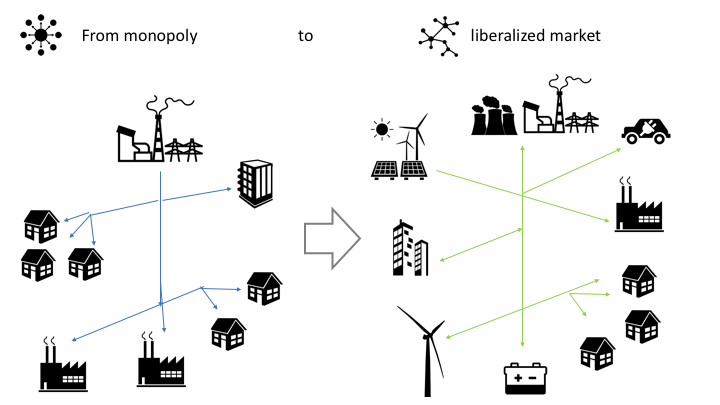
\includegraphics[width=1.00000\textwidth]{/Users/dvf/desktop/eba gitbook/Images/image13.png}

Currently, we are going through a transition on how energy markets
operate, from a centralized monopoly model to a distributed and
liberalized market.

This transition has been occurring in many countries over the last
decade, with special emphasis in the European Union.

With the growth of distributed generation, namely RES (as Wind farms,
Rooftop PV), but also with the current technologies Combined Heat and
Power Plant, plus as Storage, Electrical Cars (EV), the grid management
tends to go from top down approach to complex network management.

This market transition has occurred in parallel with an energy systems
transition, from centralized generation models to distributed generation
models.

In centralized generation systems, energy is generated in large
powerplants which are typically located away from final users.

Now, with the increasing use of different technologies, namely
renewables like wind and solar, it is possible to generate electricity
closer to final users in smaller powerplants. Ultimately, users can
themselves generate electricity for self-consumption or to inject in the
grid.

Both these transitions, which cannot be decoupled as one contributed to
the other, introduced many challenges and are reshaping the energy
sector, technologically and economically.

Grid management had to change from a model where only one company was
responsible for all activities and where all the flows had one direction
(from generation to commercialization) to a model where many companies
can operate both at the generation and commercialization, but also to a
model where the customers themselves can generate energy. So, grid
management is becoming more complex due to the existence of multiple
players and because energy flows can have two directions. Further, the
increasing use of renewables, characterized by their intermittency, as
well as new technologies like electric vehicles or storage systems,
introduces additional technical challenges.

\section{Market Players and Supply
Chain}\label{market-players-and-supply-chain}

\subsubsection{Market Players}\label{market-players}

As you recall, we are dealing with a model where all players share the
same infrastructure (the energy grid -- electricity, gas or other).

In order to this model work, besides supply and demand players, there´s
the need of regulators, Distribution and Transmission System Operators,
and entities that their role is to make sure supply always meet demand.

The main players in energy markets are:

The Governments, which are responsible for planning, and have the
ultimate responsibility to oversee that all players develop their
activity within the rules;

National Regulatory Authorities (NRAs): which are responsible for
monitoring and supervising the activities of all agents;

The Transmission System Operator (TSOs) and Distribution System Operator
(DSOs), which are the companies responsible for managing the physical
infrastructures (overhead electricity lines, pipelines, substations,
etc.) -- the transmission refers to the infrastructure in which the bulk
energy between the power plants and cities or between countries is
transported; while the distribution refers to the infrastructure in
which energy is transported between the transmission infrastructure and
the final users.

The suppliers (under regulated, liberalized market or, both), which are
responsible for supplying the energy to the energy system (powerplants,
refineries, etc)

Retailers, which are responsible for selling the energy to the final
clients;

\subsubsection{Supply Chain}\label{supply-chain}

Electricity

\begin{figure}[htbp]
\centering
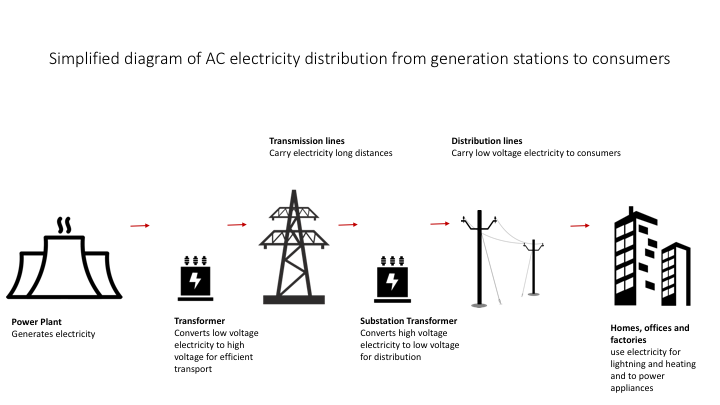
\includegraphics[width=1.00000\textwidth]{/Users/dvf/desktop/eba gitbook/Images/image14.png}
\caption{}
\end{figure}

In the case of electricity, the power plants are operated by the
suppliers. Then, the electricity is transported first through
transmission lines at very high voltage (to decrease losses) and then
through distribution lines (at high, medium or low voltage) to the final
users (homes, offices and factories). Between power plants,
transmission, distribution and final users, we have substations that are
responsible for converting the voltage and connecting the different
layers, acting therefore as infrastructures that provide safety and
security to the operation of the grid.

\subsubsection{Natural Gas}\label{natural-gas}

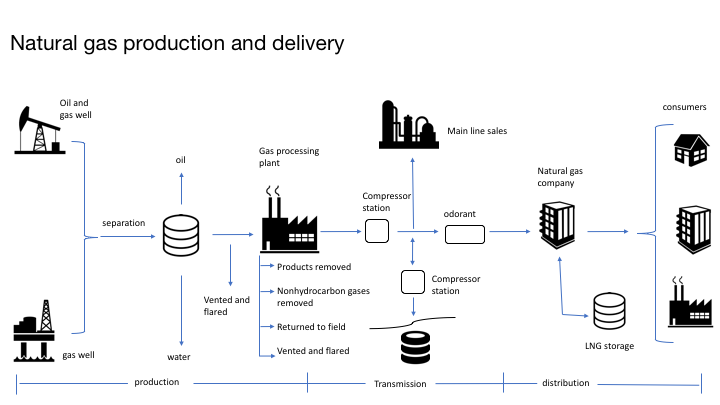
\includegraphics[width=1.00000\textwidth]{/Users/dvf/desktop/eba gitbook/Images/image15.png}
In the case of natural gas production and delivery, the players are very
similar.

The natural gas extracted at the well is transported (or stored) through
ships and pipelines. Several compression stations are placed along the
pipelines (or liquification and gasification stations in the case of
transport by ship) to guarantee the transport. Finally, the gas arrives
at the final users, which can be power plants for electricity or heat
production. One of the main difference between the electricity and
natural gas grids is that in gas it is easy to have storage elements and
therefore the match between the supply and demand is much easier to
manage.

\begin{figure}[htbp]
\centering
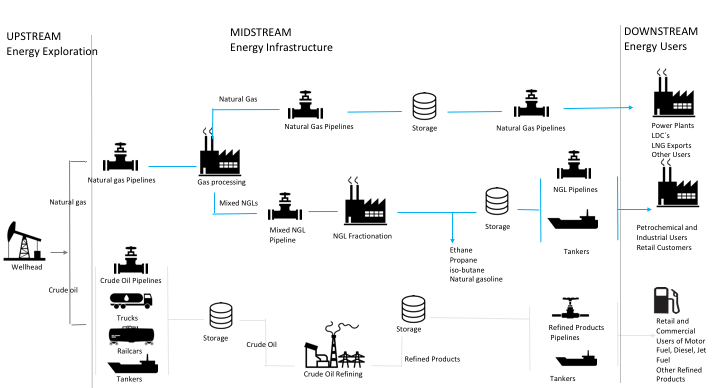
\includegraphics[width=1.00000\textwidth]{/Users/dvf/desktop/eba gitbook/Images/image16.png}
\caption{}
\end{figure}

The oil supply chain is slightly different. The core infrastructure is
the Refinery, so the transport of the raw material (crude oil) is
generally a responsibility of suppliers (extraction) and the transport
and distribution of the refined materials (diesel, gasoline, liquified
petroleum gas) is a responsibility of retailers.

Looking to combined Gas Natural and Oil, from extraction to delivery, we
still can split between production, transmission and distribution. Still
in oil \& gas you also refer as to upstream, midstream and downstream,
where:

Upstream (Exploration \& Production, which includes separation),

Midstream (Transportation \& Storage), to

Downstream (Refining, Petrochemical, \& Marketing)

As you may notice pipelines play a central role in transmission and
distribution, still unlike in electricity, you have more storage
capacity. Also most electricity is also generate using gas (and coal).

So, if you think what are the costs associated with the different energy
fuels, apart from the energy raw material (oil, gas, coal), it is
necessary to transform and to transport the energy. In the cases of
electricity and natural gas, it is necessary to consider that the
management of the transportation and distribution infrastructure
represents an additional cost, as well as cost associated with the
regulatory activities. Therefore, the cost is not only the cost of how
many kWh or m\^{}3 you consume. It is that plus all the costs related to
getting that unit of energy where it is needed, which basically covers
the costs of maintaining the reliability of the energy grid.

\section{Price for energy Components}\label{price-for-energy-components}

Looking to the final energy price, we can start by decomposing it in 3
components: energy, network and taxes and levies.

\begin{figure}[htbp]
\centering
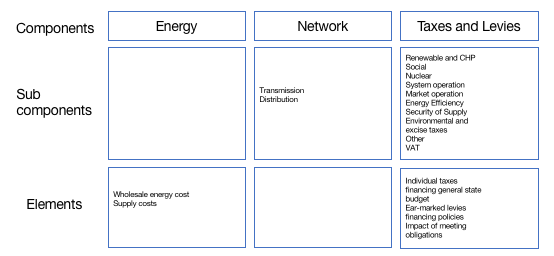
\includegraphics[width=1.00000\textwidth]{/Users/dvf/desktop/eba gitbook/Images/image17.png}
\caption{}
\end{figure}

The energy component corresponds to the costs of extracting the energy,
converting it and commercializing it and are in general charged by kwh
of consumed energy;

The network costs correspond to the costs of transporting the energy
through the infrastructure (transmission and distribution) and include
in general a part that depends on the energy consumption (kWh) but can
also depend on the power drawn from the grid (kW). It also includes a
fixed cost corresponding to the availability of supply

The Taxes and Levies costs correspond to the taxes associated with the
consumption of any good (like VAT) but also to levies, that correspond
to special payments to the government related to a very specific end.
Examples of levies are levies associated with the system operation, such
as those associated with particular energy resources (renewables,
nuclear, CHP).

\begin{figure}[htbp]
\centering
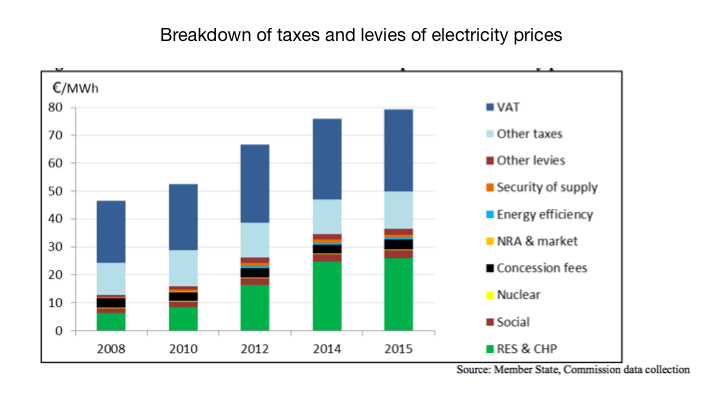
\includegraphics[width=1.00000\textwidth]{/Users/dvf/desktop/eba gitbook/Images/image18.png}
\caption{}
\end{figure}

In this chart, we see the average weight of each component in Europe and
how is has been changing over time. Considering 2008 as a baseline, and
2015, you can see a significant increase of the RES \& CHP levies of
electricity prices that mostly supported the feed-in-tariff support
mechanism of renewable technologies.

In a feed-in-tariff scheme, the renewable energy generation agents did
not have to participate in the liberalized market because they got a
fixed tariff for renewable generation, usually above market prices. This
reduced the financial risk of the investors in this project, but is has
been supported by the final users in the form of levies.

Another example are Levies in Energy Efficiency, which were also
residual in 2008, but have been gaining importance in the overall taxes
and levies of electricity prices.

IMAGE MISSING

This figure shows the electricity cost for household consumers in
European Countries in 2015. Here you can see that not only the base
energy price is different but that the taxes and levies relative weight
varies significantly, as well as the VAT.

These taxes and levies are a reflection of a country's own resources,
policies and its targets. In general, in countries that want to push
RES, they may impose either taxes on fossil fuels or subsidize RES, or a
combination of both. A country may also charge fossil fuels to penalize
their negative externalities (like CO2 emissions).

So, when analyzing the components among the different countries , you
will see the impact of such policies and choices on the energy prices.

\section{Drivers of Energy Prices}\label{drivers-of-energy-prices}

main drivers of Energy Prices, focusing on three factors: the primary
energy resource costs, the energy mix and the context (weather,
geopolitical conditions, economy).

As seen in the on energy price components, the main component in cost is
in general the energy extraction, conversion and commercialization.

The cost of the primary energy resources influences directly the cost of
energy. In general, the specific cost of fuel per unit of energy is
lower for coal than for natural gas. This is explained by the fact that
coal is a resource that is more available in nature, requires simpler
technology to extract and to transport. At this level, renewable
resources are in general the energy resources with the lowest price
(except for biomass, whose collection may present a significant cost).

The cost of primary energy resources is also affect by the existence of
this particular resource in the country or not, in which case that
country will have to import the fuel.

Regarding the conversion, the cost depends on the investment required to
install a powerplant or a refinery, the operation and maintenance costs.
Nonetheless, the final price is still largely dependent on the cost of
the fuel. In the case of electricity, natural gas power plants are more
efficient that coal power plants, require lower investments but still,
the cost of electricity produced by natural gas power plants is at the
end still more expensive than coal.

Finally, the commercialization costs may be affected by different taxes
and levies also depending on the origin.

A second factor that influences the final prices of energy is the energy
mix. The energy mix is the group of different primary energy sources
from which a final energy vector is produced. In the case of
electricity, the energy mix represents then the relative contribution of
each primary energy resource (coal, gas, renewables, nuclear and
others). If the contribution to the energy mix is mostly done by primary
resources whose cost is expensive, it will impact negatively on the
energy price. For example, countries where the electricity generation is
based on coal have generally lower energy prices than countries that use
more natural gas. Countries that have a significant share of renewables
have in principle a higher cost, not directly because of the primary
resource cost or the operation and maintenance costs, but mostly due to
the taxes and levies collected to support the operation of the system.

Finally, other factors that may influence significantly the energy
prices are the costs associated with the context, which include weather,
geopolitical conditions and the economy.

Weather is maybe the context factor that mostly affects the prices, in
many different ways. In general, cold winters will require the use of
much more heating fuels, like coal or gas and as the demand will
increase, it will make the prices higher. Reversely, if the winter are
mild, the consumption of fuels for heating will drop and the prices will
tend to decrease. However, weather also affects significantly renewable
resources. For example in countries that depend on hydro power plants,
dry years will require the use of other technologies, like gas, so the
prices will increase, while in wet years, the hydro power plants
production will be significant, so the use of other technologies will be
smaller and therefore the prices will go down.

Geopolitical conditions also affect the prices of resources: for
examples wars usually impact negatively on the prices of primary energy
resources as in general the extraction is affected.

Finally, economic conditions also affect the prices. In general, when
the economy is growing, the competition for energy resources is higher,
so the costs will increase. When we have economic crisis and the
industrial activities decrease, there is less demand and the prices tend
to go down.

So, the costs of energy depend on many different factors and that is
why, in general, an energy system -- a country or a building -- is more
robust to energy price variations if the energy mix is more diverse and
flexible.

\subsection{The EU Energy Bill}\label{the-eu-energy-bill}

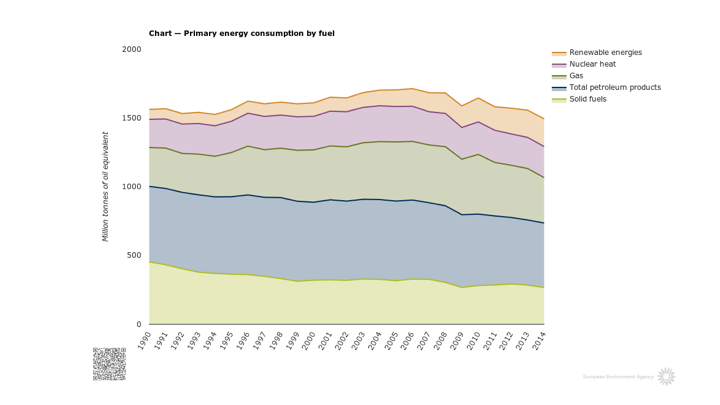
\includegraphics[width=1.00000\textwidth]{/Users/dvf/desktop/eba gitbook/Images/image20.png}
This chart gives you an idea of the relative importance of each fuel
used in different activities.

In 2014, primary energy consumption in the EU-28 countries amounted to 1
507 million tonnes of oil equivalent (Mtoe), 1.6 \% above the 2020
target.

Between 2005 and 2014, primary energy consumption in the EU-28 countries
decreased by 12 \% due to energy efficiency improvements, the increase
of the share of energy from hydro, wind and solar photovoltaics, the
economic recession and climate warming.

Fossil fuels (including non-renewable waste) continued to dominate
primary energy consumption in the EU-28, but as a proportion of total
primary energy consumption, they fell from 77.8 \% in 2005 to 71.6 \% in
2014.

The proportion of renewable energy sources almost doubled over the same
period, from 7.1 \% in 2005 to 13.4 \% in 2014, increasing at an average
annual rate of 5.8 \% per year between 2005 and 2014. The proportion of
nuclear energy in primary energy consumption was 15.0 \% in 2014.

\begin{figure}[htbp]
\centering
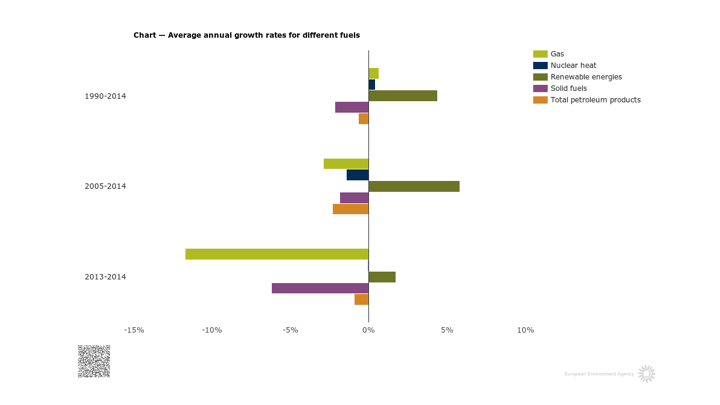
\includegraphics[width=1.00000\textwidth]{/Users/dvf/desktop/eba gitbook/Images/image21.png}
\caption{}
\end{figure}

Looking to the annual growth rates for different fuels, there is a
decrease of gas and an increases of RES.

Considering the average annual growth rates for different fuels, there
is a decrease of gas and an increases of RES. Still even having the most
average annual growth, percentage wise, looking to its absolute numbers
it is not still a main component of the energy mix.

So when looking to percentages you should take in consideration its
relative percentage too.

\begin{figure}[htbp]
\centering
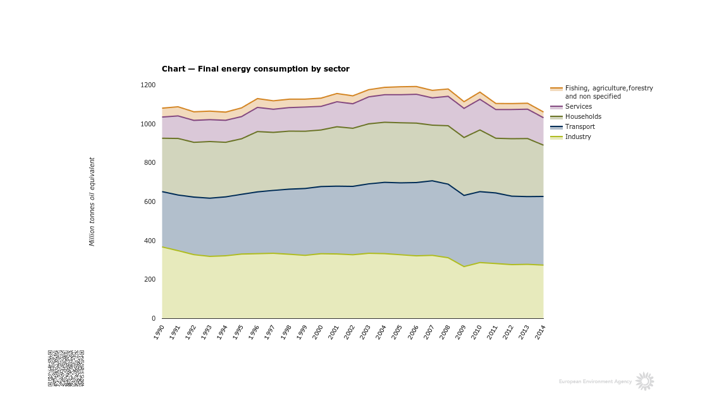
\includegraphics[width=1.00000\textwidth]{/Users/dvf/desktop/eba gitbook/Images/image22.png}
\caption{}
\end{figure}

As you may be aware there are 3 main sectors: as transportation,
industry, households.

Considering the Final energy consumption of petroleum products by
sector, most part is used in transportation,

In Final energy consumption of natural gas by sector, households and
industry are the two main sectors and

Electricity is mostly used by households, industry and services.

Buildings most are allocated to households and services sectors.

\begin{figure}[htbp]
\centering
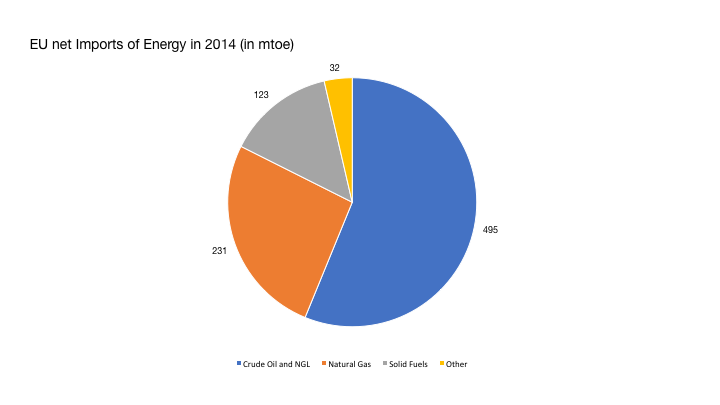
\includegraphics[width=1.00000\textwidth]{/Users/dvf/desktop/eba gitbook/Images/image19.png}
\caption{}
\end{figure}

High import dependency means that the EU faces an important energy
import bill.

In 2013, the EU's estimated import bill reached EUR 400 billion. Since
then, falling energy prices allowed the import bill to fall
significantly, although the weakening of the euro has partly offset this
effect.

In 2015, the estimated import bill amounted to EUR 261 billion, 35\%
less than in 2013. In 2 years, the import bill decreased by EUR 142
billion, about 1\% of EU GDP, thereby giving a significant boost to the
economy.

Crude oil is by far the main component of the import bill, making up
68\% of the total in 2015.

The share of gas and hard coal was 28\% and 4\%, respectively.

Russia is the main supplier of all three fossil fuels: crude oil,
natural gas and hard coal. In 2015, 34\% of the import bill went to
Russia. Russia was followed by Norway (19\%) and Nigeria (7\%).

The import bill basically depends on the volume and the average price of
imports. Like most commodities, energy sources are typically traded in
US dollars and therefore the development of the USD/EUR exchange rate
will also influence the import bill (if expressed in euros). ''

\subsection{Demand Side Management}\label{demand-side-management}

Until now we only refereed annual demand and supply. Still there is no
perfect match with supply or demand or can easily shift supply forward,
to when will be a higher consumption.

\begin{figure}[htbp]
\centering
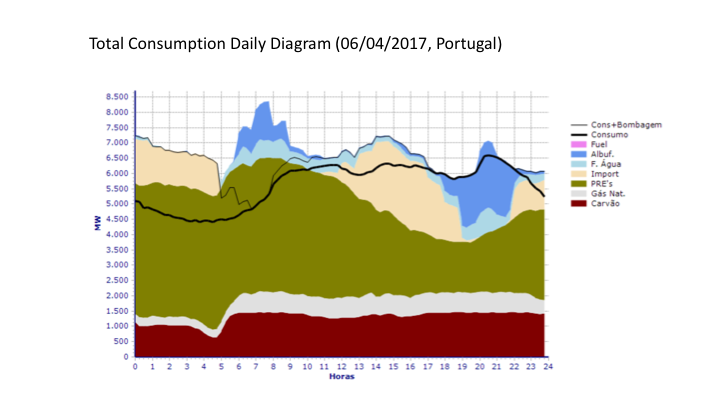
\includegraphics[width=1.00000\textwidth]{/Users/dvf/desktop/eba gitbook/Images/image23.png}
\caption{}
\end{figure}

Taking for example the total daily Consumption diagram gives you
important information as:

Total Consumption; Total supply; Excess or deficient of supply at a
given time and; Imports or exports due to the last.

You may notice two peaks, one in the morning and other around late
evenings. If you think about you daily routines, including factories and
services, it´s much a reflection of people´s activities, where during
late nights you consumption decreases.

\begin{figure}[htbp]
\centering
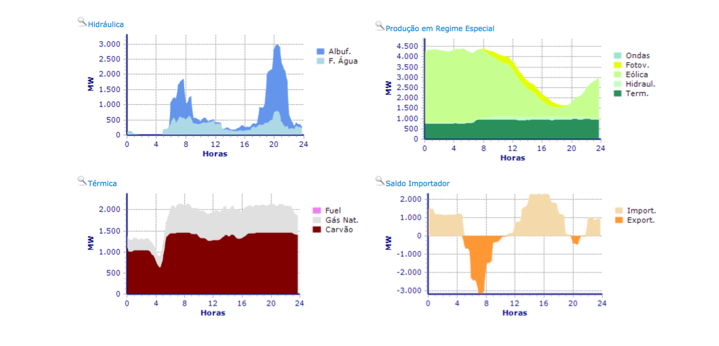
\includegraphics[width=1.00000\textwidth]{/Users/dvf/desktop/eba gitbook/Images/image24.png}
\caption{}
\end{figure}

If you breakdown demand you will also notice that supply varies quite
differently depending on each source, where solar has a peak around
midday, wind late nights, hydro depends on weather and availed capacity,
combustion plants most of the times needs a lot of hours to be in full
steam and are also used as a backup system, when RES are not available.

RES has the problem of intermittency, so until can secure that supply
always meet demand, grid operators have the task:

Securing supply to match demand; Trying to match and manage all
available energy sources, according to timely and future needs;
real-time dispatch of generation and managing security

The role of the System Operator in a wholesale market is to manage the
security of the power system in real time and co-ordinate the supply of
and demand for electricity, in a manner that avoids fluctuations in
frequency or interruptions of supply.

Balancing demand and supply:

Securing supply to match demand;

Trying to match and manage all available energy sources, according to
timely and future needs;

Real-time dispatch of generation and managing security

This can be achieved by:

\begin{itemize}
\tightlist
\item
  Determining the optimal combination of generating stations and reserve
  providers for each market trading period,
\item
  instructing generators when and how much electricity to generate, and
  -Managing any contingent events that cause the balance between supply
  and demand to be disrupted.
\end{itemize}

You have to also take into account factor behind changes in energy
consumption, witch changes across countries, such as: Change in Total
Consumption. Consumption habit change; Increase in household stock and
appliances Energy Savings

\begin{figure}[htbp]
\centering
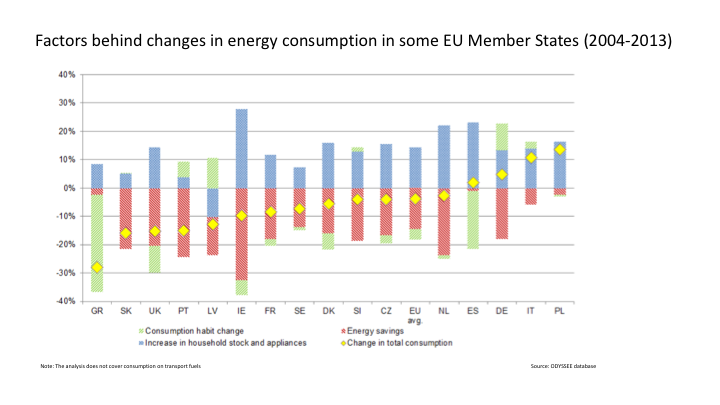
\includegraphics[width=1.00000\textwidth]{/Users/dvf/desktop/eba gitbook/Images/image25.png}
\caption{}
\end{figure}

As you may notice there is an overall increase in Increase in household
stock and appliances

\begin{figure}[htbp]
\centering
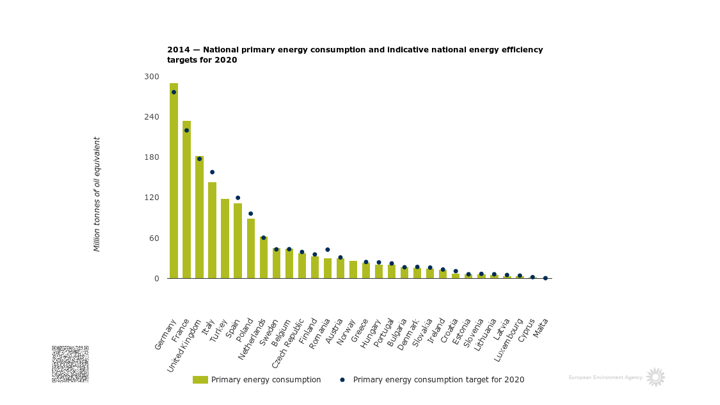
\includegraphics[width=1.00000\textwidth]{/Users/dvf/desktop/eba gitbook/Images/image26.png}
\caption{}
\end{figure}

And Energy Savings. A change in consumers habits tend to be hard to
implements or promote incentive to that change.

As one way to incentive EE, there each country defined its indicative
national energy efficiency targets for 2020

Currently some country already fulfilled those targets, namely Germany
and France. Other don´t.

Real time monitoring (smart meters) to:

\begin{quote}
Provide information to Shift consumption patterns to match supply
\end{quote}

For example, one of the important pieces to promote EE measures is real
time monitoring, or providing users with smart meters.

This would enable real time monitoring to either provide information to
either human or machines to adapt consumption to market (supply).

Demand Side Management, needs that information available in forms that
can be used to make decisions on when and how much energy purchase. So
when referring demand side management, means doing the best allocation
of resources (price) to needs (quantity), considering that prices varies
depending on supply and some consumption - the demand - can be deferred
to moments where there is abundance of supply.

\subsection{Dynamic Pricing and Intervention in Prices setting
Mechanisms}\label{dynamic-pricing-and-intervention-in-prices-setting-mechanisms}

Several methods of dynamic pricing exist, depending on two main factors:

\begin{verbatim}
(i) the granularity of the period during which consumption is metered separately, and

(ii) the dynamics/statics of Time-of-Use (ToU) prices.
\end{verbatim}

The impact on consumers (who can be rewarded for adapting their energy
consumption to price signals, but can also be penalised if they continue
to consume at peak times) depends on the combination of these two
factors, i.e. ``dynamic pricing application'', for instance:

\begin{verbatim}
a) “static ToU” is a dynamic pricing application in which fixed time bands are set and the price for each time band reflects the average wholesale price in the time band (low granularity-low dynamics). Although less common, a high granularity-low dynamics application is possible, where hourly consumption is priced at monthly average prices;

b) “critical peak pricing” is a dynamic pricing application in which a higher price is charged in limited periods when the consumption peak at the system level occurs (low granularity-high dynamics); and

c) “real-time pricing” is a dynamic pricing application in which the price is posted in real time and communicated to the consumer (high granularity-high dynamics).
\end{verbatim}

There are several Dynamic pricing mechanism, with several levels of
granularity.

\begin{figure}[htbp]
\centering
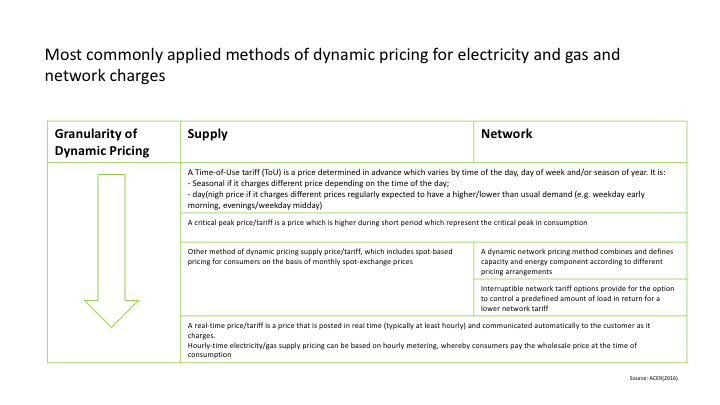
\includegraphics[width=1.00000\textwidth]{/Users/dvf/desktop/eba gitbook/Images/image27.png}
\caption{}
\end{figure}

\begin{figure}[htbp]
\centering
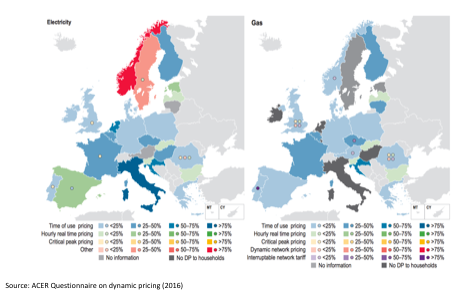
\includegraphics[width=1.00000\textwidth]{/Users/dvf/desktop/eba gitbook/Images/image28.png}
\caption{}
\end{figure}

Where time of use pricing, in blue, is quite prevalent if you consider
the Share of standard household consumers supplied under dynamic pricing
for supply and network charges of electricity in EU MSs -- 2015 (\%),
percentage wise.

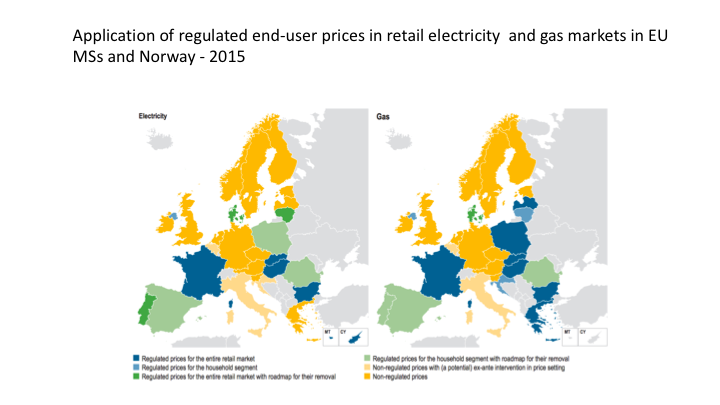
\includegraphics[width=1.00000\textwidth]{/Users/dvf/desktop/eba gitbook/Images/image29.png}
If you look to the application of regulated end-user prices in retail
electricity and gas markets in the EU and Normay, in 2015, there is
still a combination of:

Regulated prices for the entire retail market Regulated prices for the
household segment Regulated prices for the entire retail market with
roadmap to their removal Regulated prices for the household segment with
roadmap to their removal

And

Non regulated prices with (a potential) ex-ante intervention in price
setting Non-regulated prices

Where, in electricity and gas markets, Non-regulated prices, Regulated
prices for the household segment with roadmap to their removal and
Regulated prices for the entire retail market are the most common.

\begin{figure}[htbp]
\centering
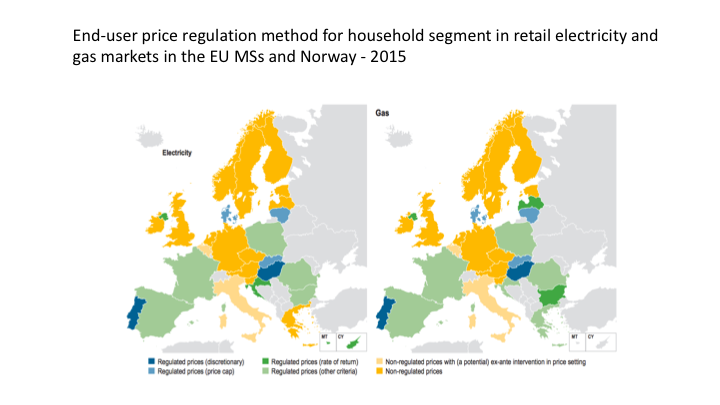
\includegraphics[width=1.00000\textwidth]{/Users/dvf/desktop/eba gitbook/Images/image30.png}
\caption{}
\end{figure}

If you remember, as refereed in a previously, infrastructure access'
prices plays a central role in energy markets.

So when setting the method for End-user you can see the connection with
the , infrastructure access' prices and regulation method for the
household segment.

Where you see: Regulated prices (discretionary); Regulated prices (price
cap, for example by setting maximum \% increase, usually indexed to some
economic indicator, as Consumer Index Price, Inflation) Regulated prices
(rate of return, this one can also be design as the minimum rate return
for the utility has to have, scheme quite common in Portugal, not only
in utilities, but also for other PPP) Regulated prices (other criteria)

And

Non-regulated prices with (a potential) ex-ante intervention in price
setting; Non regulated prices;

Specially in household segment there there´s special provisions to
access to basic good and services, as energy is.

On Network tariffs, the Energy Efficiency Directive states Network or
retail tariffs may support dynamic pricing for demand response measures
by final customers, such as:

\begin{enumerate}
\def\labelenumi{(\alph{enumi})}
\tightlist
\item
  time-of-use tariffs;
\item
  critical peak pricing;
\item
  real time pricing; and
\item
  peak time rebates.
\end{enumerate}

It also states that network tariffs shall be cost effective of cost
savings in networks.

Also, network tariffs shall not prevent:

\begin{enumerate}
\def\labelenumi{(\alph{enumi})}
\tightlist
\item
  the shifting of the load from peak to off-peak times by final
  customers;
\item
  energy savings from demand response of distributed consumers by energy
  aggregators;
\item
  demand reduction from energy efficiency measures undertaken by energy
  service providers, including energy service companies;
\item
  the connection and dispatch of generation sources at lower voltage
  levels;
\item
  the connection of generation sources from closer location to the
  consumption; and
\item
  the storage of energy.
\end{enumerate}

Chart 1 - Real GDP growth rate

\begin{figure}

{\centering \includegraphics[width=0.8\linewidth]{EBA_Notes_files/figure-latex/r gdp-fig-1} 

}

\caption{GDP}(\#fig:r gdp-fig)
\end{figure}

\chapter{Project Management}\label{project-management}

\section{Basic Concepts}\label{basic-concepts}

\subsection{Economic and financial
dimensions}\label{economic-and-financial-dimensions}

Projects evaluation can be described as a methodology for assessing the
economic and financial (and social and environmental) impact of a
proposed investment.

Project evaluation should focus on two dimensions:

\begin{itemize}
\item
  An \textbf{Economic analysis}, which is a systematic approach to
  determine the optimum use of resources (capital, human resources) and
  it involves the comparison of two or more alternatives to achieve a
  specific objective under certain assumptions and constraints. In
  particular, it attempts to measure in monetary terms the costs and
  benefits of the project to the organization or the community or
  economy.
\item
  A \textbf{Financial analysis}, which aims to determine the financial
  resources to develop the project, like choosing the funding sources
  (equity or debt).
\end{itemize}

When we refer to the economic analysis of a project, we are most of the
times referring to the idea of the Opportunity Cost of a given decision.

\subsection{Opportunity cost}\label{opportunity-cost}

The opportunity cost is the benefit or value that you give up by
choosing one option over another. In other words, the opportunity cost
of a decision is the difference between the value you receive from
pursuing a certain option and the value that you would have received
from the alternative that you chose not to pursue.

We can express opportunity cost in terms of a return (or profit) on
investment by using the following mathematical formula:

\[Opportunity Cost = Return on Most Profitable Investment Choice - Return on Investment Chosen to Pursue\]

Unless the investment returns are fixed and guaranteed to be paid (like
a Treasury bond you intend to hold to maturity), you'll have to base
your calculation on the expected returns.

Example: imagine you want to buy an efficient equipment.

You have two potential options:

\begin{itemize}
\tightlist
\item
  Change lighting system to LED (20\% return on investment)or
\item
  installing a PV system (10\% return on investment).
\end{itemize}

The opportunity cost is the difference between the benefits you would
get from the one option (e.g.~Change lighting system to LED) over
another (installing a PV system).

What is the opportunity cost?

If you decide to leave install a new PV system, the opportunity cost is:

20\% (changing the lighting system) - 10\% (installing the pv system,
option that is being pursuit) = 10\%

This is your trade off for choosing one option instead of another.

\subsection{Time value of money}\label{time-value-of-money}

When dealing with financial investments one of the basic underlying
issues emerges from answering the question:

\begin{quote}
Do you prefer to have 100\euro{} today or invest 100\euro{} for a future
income?
\end{quote}

The idea of time is quite fundamental in finance, because in general,
the money available at the present time is worth more than the same
amount in the future, due to its potential earning capacity.

Time value of money can reflect that a certain amount of money today has
a different buying power (value) than the same currency amount of money
in the future, but is not an equivalent.

If you consider as geometric series, the first term would be the present
value, the common ratio would be (1+i) and n, number of periods.

So we start by this basic formula:

\[Future\ Value = Present Value \cdot (1+i)^n\]

Or the present Value of a certain amount of money C (at n year) is given
by:

\[Present\ Value = \frac{C}{(1+i)^n}\]

Cash Flow C - Net amount of money that goes in or out of a project

If we want to estimate how much is the Present value of a certain future
cash flows C that will be collected in the future ``n'' year,\\
where n is the number of compounding periods between the present date
and the date where the sum is worth C i is the interest rate for one
compounding period (the end of a compounding period is when interest is
applied, for example, annually, semiannually, quarterly, monthly,
daily).

(The interest rate i is given as a percentage, but expressed as a
decimal in this formula. If using periods with less than one year, for
example 6 month would be power of ½ or 6/12)

Compounding is the process where the value of an investment increases
because the earnings on an investment, both capital gains and interest,
earn interest as time passes. This exponential growth occurs because the
total growth of an investment along with its principal earn money in the
next period. This differs from linear growth, where only the principal
earns interest each period.

If you consider as geometric series, the first term would be the present
value, the common ratio would be (1+i) and n, number of periods

Figure 1 - Geometric growth

\begin{figure}[htbp]
\centering
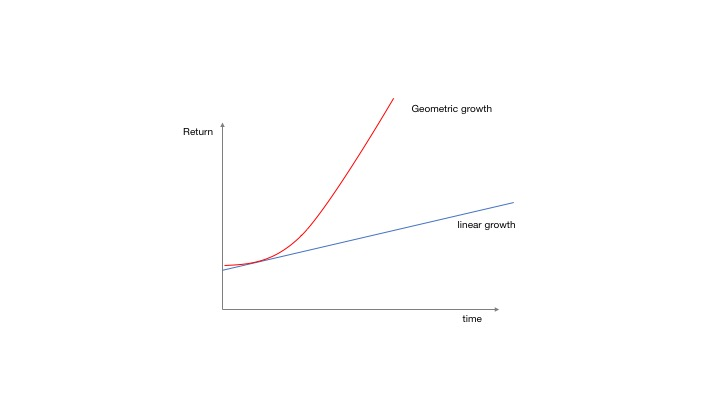
\includegraphics[width=1.00000\textwidth]{/Users/dvf/desktop/eba gitbook/Images/image1.jpg}
\caption{}
\end{figure}

If you notice, more than the interest rate, times plays a central role,
or what so called the power compound interest, so you are dealing with
geometric growth, not linear and the reasoning can be linked to the idea
of trade-offs. You will defer consumption today, to have a certain
return in n years, but because you just will have that return in n years
it is like if you were reinvesting every year.

Example:

year 0, you have 100\euro{}, year 1, you would have 100+1.10 (10\%
rate), year 2, you start with 110 (and not 100 \euro{}) so you will have
121 (110*1.1) and so on.

Another way to put is:

What is would you choose? 1) 100\euro{} today or; 2) 103\euro{} in 1
year

If you consider a 4\% interest rate

We would level both options with the previous formula

So option 1 would be equivalent to: \(100 \times (1.04)^1\) or
104\euro{}

or doing for present value \(C_0 =103/104 = 99€\)

So 100\euro{} are equal to 104\euro{} in 1 year and 103\euro{} in 1 year
time is equivalent to 99\euro{} today.

The time value of money is the assumption that money can generate value
if it is invested (for example interests in a bank), so it is better to
receive the money now than later.

At the end, the same amount of money today has a different and higher
buying power (value) than the same amount of money in the future, it is
not an equivalent.

The rate at which the money is appreciate or depreciate is called the
discount rate. This discount rate may represent different factors but is
often considered to be the interest rate given by the treasury bounds of
central banks at 10 years, usually are used as benchmark (risk free) to
computed riskier investments. It is often represented by the letter
``i'' of interest.

Example 2

1010=1000x(1+0.01), with n=1

Imagine that you have 1000\euro{} and you put in the bank with a 1\%
interest rate. In one year, the 1000 euros you have today will be worth
1010\euro{}.

In 2 years it will be worth 1020.1\euro{}.

Cash Flow C - Net amount of money that goes in or out of a project If we
want to estimate how much is the Present value of a certain future cash
flows C that will be collected in the future ``n'' year, we can invert
the future value formula and obtain the present value formula:

Time of value example

990.01=1000/(1+0.01), with n=1 Imagine that you have the opportunity to
collect 1000\euro{} in one year.

That is equivalent to receiving today only 990.01 \euro{} (because if
you put in the bank today 990.01 \euro{}), you will have 1000 euros next
year.

\subsection{Money}\label{money}

Money can also be defined as:

\begin{itemize}
\tightlist
\item
  It's a store of value, meaning that money allows you to defer
  consumption until a later date.
\item
  It's a unit of account, meaning that it allows you to assign a value
  to different goods without having to compare them. So instead of
  saying that a car is worth ten cows, you can just say it (or the cows)
  cost 10 000 \euro{}.
\item
  And it's a medium of exchange---an easy and efficient way for you and
  me and others to trade goods and services with one another.
\end{itemize}

The idea that a euro today is worth more than a euro tomorrow, relates
more to the second and last roles, storage and medium of exchange,
because the value of money at a future point of time would take account
of interest earned and the inflation accrued over a given period of
time.

Inflation is the rate at which the general level of prices for goods and
services is rising and, consequently, the purchasing power of currency
is falling. Central banks attempt to limit inflation, and avoid
deflation, in order to keep the economy running smoothly, namely by
setting interest rates.

\section{Indicators}\label{indicators}

Basic indicators that should be computed to evaluate a project and aid
in the decision of developing it or not: net present value, internal
rate of return and payback period.

\subsection{Net Present Value (NPV)}\label{net-present-value-npv}

The first indicator to evaluate a project, is the Net Present Value
(NPV), which basically estimates the value that will be gained at
present costs by developing the project. This estimate consists in
adding all future net earnings (the cashflows) minus the initial
investment that is required to execute the project.

\[NPV_{i, N}  \sum_{n=0}^{N}\frac{C_n}{(1+i)^n} - Investment\]

Net present value (NPV) of a project is the potential change in an
investor's wealth caused by that project while time value of money is
being accounted for. It equals the present value of net cash inflows
generated by a project less the initial investment on the project. It is
one of the most reliable measures used in capital budgeting because it
accounts for time value of money by using discounted cash flows in the
calculation.

Net present value calculations take the following two inputs: Projected
net cash flows in successive periods from the project. A target rate of
return i.e.~the discount rate.

Where,

Net cash flow equals total cash inflow during a period, including
salvage value if any, less cash outflows from the project during the
period.

Hurdle rate is the rate used to discount the net cash inflows. Weighted
average cost of capital (WACC)is the most commonly used discount rate.

\begin{figure}[htbp]
\centering
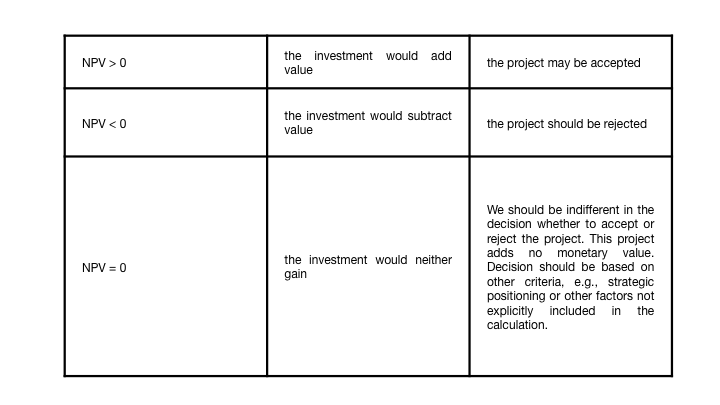
\includegraphics[width=1.00000\textwidth]{/Users/dvf/desktop/eba gitbook/Images/image2.png}
\caption{}
\end{figure}

NPV (even and uneven)

Calculation Methods and Formulas

The first step involved in the calculation of NPV is the estimation of
net cash flows from the project over its life. The second step is to
discount those cash flows at the hurdle rate.

NPV (even and uneven)

The net cash flows may be even (i.e.~equal cash flows in different
periods) or uneven (i.e.~different cash flows in different periods).

When they are even, present value can be easily calculated by using the
formula for present value of annuity. However, if they are uneven, we
need to calculate the present value of each individual net cash inflow
separately. Once we have the total present value of all project cash
flows, we subtract the initial investment on the project from the total
present value of inflows to arrive at net present value.

Thus we have the following two formulas for the calculation of NPV:

When cash inflows are even: NPV = R × 1 − (1 + i)-n − Initial Investment

In the above formula, R is the net cash inflow expected to be received
in each period; i is the required rate of return per period; n are the
number of periods during which the project is expected to operate and
generate cash inflows.

When cash inflows are uneven: NPV =

R1 + R2 + R3 + \ldots{}

− Initial Investment

(1 + i)1

(1 + i)2

(1 + i)3

Where, i is the target rate of return per period; R1 is the net cash
inflow during the first period; R2 is the net cash inflow during the
second period; R3 is the net cash inflow during the third period, and so
on \ldots{}

Decision Rule In case of standalone projects, accept a project only if
its NPV is positive, reject it if its NPV is negative and stay
indifferent between accepting or rejecting if NPV is zero. In case of
mutually exclusive projects (i.e.~competing projects), accept the
project with higher NPV.

Examples Example 1: Even Cash Inflows: Calculate the net present value
of a project which requires an initial investment of \$243,000 and it is
expected to generate a cash inflow of \$50,000 each month for 12 months.
Assume that the salvage value of the project is zero. The target rate of
return is 12\% per annum. Solution We have, Initial Investment =
\$243,000 Net Cash Inflow per Period = \$50,000 Number of Periods = 12
Discount Rate per Period = 12\% ÷ 12 = 1\% Net Present Value = \$50,000
× (1 − (1 + 1\%)\^{}-12) ÷ 1\% − \$243,000 = \$50,000 × (1 −
1.01\^{}-12) ÷ 0.01 − \$243,000 ≈ \$50,000 × (1 − 0.887449) ÷ 0.01 −
\$243,000 ≈ \$50,000 × 0.112551 ÷ 0.01 − \$243,000 ≈ \$50,000 × 11.2551
− \$243,000 ≈ \$562,754 − \$243,000 ≈ \$319,754

Example 2: Uneven Cash Inflows: An initial investment of \$8,320
thousand on plant and machinery is expected to generate cash inflows of
\$3,411 thousand, \$4,070 thousand, \$5,824 thousand and \$2,065
thousand at the end of first, second, third and fourth year
respectively. At the end of the fourth year, the machinery will be sold
for \$900 thousand. Calculate the net present value of the investment if
the discount rate is 18\%. Round your answer to nearest thousand
dollars. Solution PV Factors: Year 1 = 1 ÷ (1 + 18\%)\^{}1 ≈ 0.8475 Year
2 = 1 ÷ (1 + 18\%)\^{}2 ≈ 0.7182 Year 3 = 1 ÷ (1 + 18\%)\^{}3 ≈ 0.6086
Year 4 = 1 ÷ (1 + 18\%)\^{}4 ≈ 0.5158 The rest of the calculation is
summarized below: Year 1 2 3 4 Net Cash Inflow \$3,411 \$4,070 \$5,824
\$2,065 Salvage Value

900 Total Cash Inflow \$3,411 \$4,070 \$5,824 \$2,965 × Present Value
Factor 0.8475 0.7182 0.6086 0.5158 Present Value of Cash Flows
\$2,890.68 \$2,923.01 \$3,544.67 \$1,529.31 Total PV of Cash Inflows
\$10,888

− Initial Investment − 8,320

Net Present Value \$2,568 thousand

Strengths and Weaknesses of NPV

Strengths Net present value accounts for time value of money which makes
it a sounder approach than other investment appraisal techniques which
do not discount future cash flows such payback period and accounting
rate of return. Net present value is even better than some other
discounted cash flows techniques such as IRR. In situations where IRR
and NPV give conflicting decisions, NPV decision should be preferred.

Weaknesses NPV is after all an estimation. It is sensitive to changes in
estimates for future cash flows, salvage value and the cost of capital.
Net present value does not take into account the size of the project.
For example, say Project A requires initial investment of \$4 million to
generate NPV of \$1 million while a competing Project B requires \$2
million investment to generate an NPV of \$0.8 million. If we base our
decision on NPV alone, we will prefer Project A because it has higher
NPV, but Project B has generated more shareholders' wealth per dollar of
initial investment (\$0.8 million/\$2 million vs \$1 million/\$4
million).

\subsection{Internal Rate of Return
(IRR)}\label{internal-rate-of-return-irr}

The Internal Rate of Return (IRR), corresponds to finding out what is
the rate of return of the project that makes the NPV equal to 0.

\[IRR=  \sum_{n=0}^{N}\frac{C_n}{(1+i)^n} = 0\]

Imagine you want to develop this project, but one of two things may
happen:

\begin{enumerate}
\def\labelenumi{\arabic{enumi})}
\tightlist
\item
  you need to go to a bank, ask for a loan and will have to pay an
  interest rate of 5\%;
\item
  you need to take the money from the bank and will loose a 5\% interest
  rate.
\end{enumerate}

If the IRR is higher than this (5\%), it means you should develop the
project, as the value that you will get from the project is higher that
what you need to invest.

\subsection{Payback Period}\label{payback-period}

Lastly, sometimes you want to know how much is the period of time
required for the return on an investment to ``repay'' the sum of the
original investment.

So the simple formula to answer that question is given as:

\[Payback \, Period = \frac{Amount\,Invested}{Estimated\,Net\,Cash\,Flow}\]

The payback can be calculated in a simplified way -- where the time
value of money is not taken into account - or in a discounted way, where
the net cash flows are calculated using the present cost (discounted
payback period).

Project evaluation should never be only based on the analysis of one
single indicator. Only the combined analysis of all indicators, will
provide enough information to take a well informed decision.

\section{Cash Flows}\label{cash-flows}

\subsection{Nature}\label{nature}

As we mention, the cashflow is the net balance between positive and
negative money flows in the project. When we are dealing with project
evaluation we can split the money flows between costs and revenues, by
nature in the following categories:

Investment, Operating Financing

The investment costs are related to how much is it necessary to spend to
generate future revenues. In the energy field, this is the investment
necessary to increase energy savings (e.g.~changing the lighting system
or install a new monitoring system) or eventually to get some revenue
(e.g.~Installing a PV system that can back sell to the grid the excess)

The cash flow is the net balance of all the revenues and costs,
regardless of their nature (financing, operating or investment)

In a project evaluation it should be always positive, as it means that
the revenues are larger than the expenses.

\subsection{Fix costs and variable
costs}\label{fix-costs-and-variable-costs}

You also can spilt by:

Fix costs and variable costs.

A variable cost and fixed cost are the two main costs a company has when
producing goods and services. A company's total cost is composed of its
total fixed costs and its total variable costs. Variable costs vary with
the amount produced. Fixed costs remain the same, no matter how much
output a company produces.

\begin{figure}[htbp]
\centering
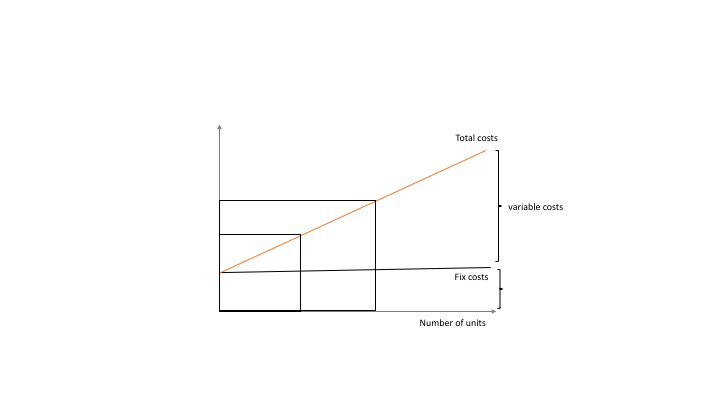
\includegraphics[width=1.00000\textwidth]{/Users/dvf/desktop/eba gitbook/Images/imagem3.png}
\caption{}
\end{figure}

A variable cost is a company's cost that is associated with the amount
of goods or services it produces. A company's variable cost increases
and decreases with the production volume. For example, suppose company
ABC produces ceramic mugs for a cost of \$2 a mug. If the company
produces 500 units, its variable cost will be \$1,000. However, if the
company does not produce any units, it will not have any variable cost
for producing the mugs.

On the other hand, a fixed cost does not vary with the volume of
production.

A fixed cost does not change with the amount of goods or services a
company produces. It remains the same even if no goods or services are
produced. Using the same example above, suppose company ABC has a fixed
cost of 10,000 per month for the machine it uses to produce mugs. If the
company does not produce any mugs for the month, it would still have to
pay 10,000 for the cost of renting the machine. On the other hand, if it
produces 1 million mugs, its fixed cost remains the same. The variable
costs change from zero to \$2 million in this example.

value of money that has been used up to produce something, and hence is
not available for use anymore Investment costs -- value used to buy an
asset required to the project Operation costs -- value used to operate
the asset required to the project Fixed costs -- value of money spent
because there is a project going on

\subsection{Break even analysis}\label{break-even-analysis}

We can relate Total Costs and its Fix and Variable Costs to answer a
simple question:

How many units do I have to sale to pay for the Fix Costs? Or to Break
even?

\begin{figure}[htbp]
\centering
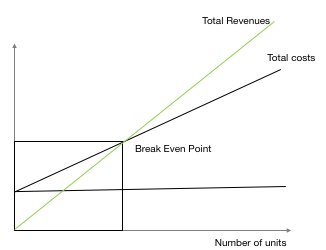
\includegraphics[width=1.00000\textwidth]{/Users/dvf/desktop/eba gitbook/Images/image4.png}
\caption{}
\end{figure}

\[Fixed \ Costs ÷ (Price - Variable Costs) = Breakeven\ Point\ in \ Units\]

Where you divide the Fix Costs by the difference between Price and
Variable Costs, that can also the the Cost of goods Sold,

The result is the Breakeven Point in Units, meaning how many units you
have to sell to pay for the fix Costs.

\begin{figure}[htbp]
\centering
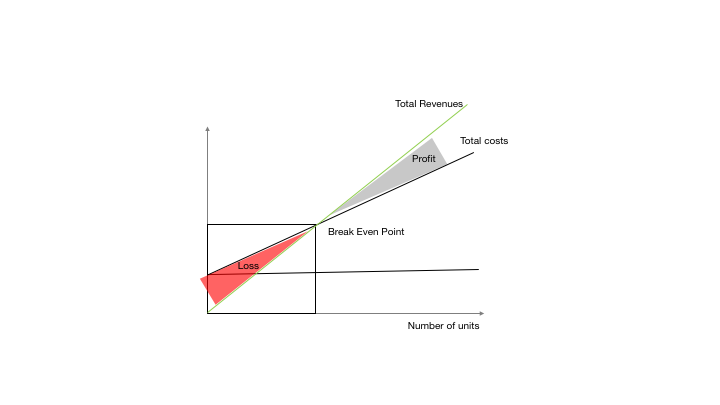
\includegraphics[width=1.00000\textwidth]{/Users/dvf/desktop/eba gitbook/Images/image5.png}
\caption{}
\end{figure}

If you look to the graph, you can see the BEP, or the equilibrium point
of the Total revenues curve and Total Cost Curve, where any value on the
left, mean that you be in loss region, and on the right profitable
region.

\subsection{Cash Flows in EE}\label{cash-flows-in-ee}

In energy efficiency, the cash flows have a special nature as they in
general they do not represent a real money inflow to the company, but
rather a smaller expense or outflow. When we implement an energy
efficiency measure, we do not receive money for it (except in few cases,
like selling electricity to the grid), but we spend less money in
energy.

Most will assume that savings, namely in EE projects are equal to future
earnings (or a future stream of cash flows), but you should be aware
that is not, namely:

Savings means fewer costs, not more revenues;

Means that unless you take those savings and invest in a similar project
with a similar stream of cash flows, you can´t compound negative value
(or for simplicity, assume that you can only compound values greater
than 0).

You will have to make payments in the future, namely if under a EPC
Contract, so when looking to an EE investment you better consider as an
investment, where you may have to pay something upfront the rest delayed
in future payment and in the future (after payment the investment) you
will have to use fewer funds for energy.

\begin{figure}[htbp]
\centering
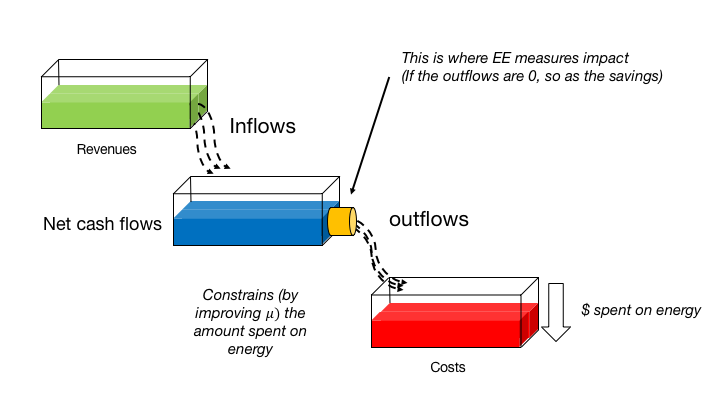
\includegraphics[width=1.00000\textwidth]{/Users/dvf/desktop/eba gitbook/Images/image6.png}
\caption{}
\end{figure}

So you can consider as net flows of inflows and outflows of money, where
EE measure will impact the outflows, still, if the outflows are 0 (you
don't spend any in energy, means that you will have 0 savings because
there's no efficiency to apply to outflows.

\subsection{Financial Statements}\label{financial-statements}

The Relationship Between the Financial Statements

The income statement, balance sheet and cash flow statement are all
interrelated.

The income statement describes how the assets and liabilities were used
in the stated accounting period.

The cash flow statement explains cash inflows and outflows, and it will
ultimately reveal the amount of cash the company has on hand, which is
also reported in the balance sheet. By themselves, each financial
statement only provides a portion of the story of a company's financial
condition; together, they provide a more complete picture.

In the context of corporate financial reporting, the income statement
summarizes a company's revenues (sales) and expenses, quarterly and
annually for its fiscal year. The final net figure, as well as various
other numbers in the statement, are of major interest to the investment
community.

Multi-Step Format Single-Step Format Net Sales Net Sales Cost of Sales
Materials and Production Gross Income* Marketing and Administrative
Selling, General and Administrative Expenses (SG\&A) Research and
Development Expenses (R\&D) Operating Income* Other Income \& Expenses
Other Income \& Expenses Pretax Income Pretax Income* Taxes Taxes Net
Income Net Income (after tax)* --

\subsection{Investments}\label{investments}

A capital expenditure, or CAPEX, is considered an investment into the
business. The money spent is not immediately reported on the income
statement; rather, it is treated as an asset on the balance sheet. A
CAPEX is deducted over the course of several years as a depreciation
expense, beginning with the year following the purchase. The
depreciation expense is reported on the income statement in the tax
years it is deducted, resulting in reduced profit.

For example, say you own a flower shop and in 2012, you purchase a
delivery van for \$30,000. The van is recorded as an asset on 2012's
balance sheet, leaving the income statement for 2012 unaffected by the
purchase. You expect to use the van for six years, so it is depreciated
by \$5,000 each year. So, on 2013's income statement, a \$5,000 expense
is then reported. While a CAPEX does not directly affect income
statements in the year of purchase, for each subsequent year for the
expected useful life of the asset the depreciation expense affects the
income statement. A CAPEX may indirectly have an immediate effect on
income statements depending on the type of asset that is acquired. Using
the previous example, the van purchased for the flower shop is not
recorded on the income statement for 2012, but gas and insurance
expenses for the van are considered business expenses that affect the
income statement. However, the expenses incurred by the van may be
offset by the increase in revenue produced by the delivery van.

The term cash and cash equivalents includes: currency, coins, checks
received but not yet deposited, checking accounts, petty cash, savings
accounts, money market accounts, and short-term, highly liquid
investments with a maturity of three months or less at the time of
purchase such as U.S. treasury bills and \ldots{}

A cash position represents the amount of cash that a company, investment
fund or bank has on its books at a specific point in time. The cash
position is a sign of financial strength and liquidity. In addition to
cash itself, this position often takes into consideration highly liquid
assets, such as certificates of deposit, short-term government debt and
other cash equivalents.

\subsection{Loan}\label{loan}

Principal + interest

\subsection{Capital Structure}\label{capital-structure}

The way you decide to finance the project (Capital Structure) plays a
central role in Financial Analysis.

EV

BOX

You can use an opportunity cost analysis to help you decide how to best
capitalize a project. A project' capital structure is simply how a
company finances its operations. Capital structure may involve a mix of
debt (long-term or short-term) and equity, and Equity, which is the
infusion of capital into a business using the company's resources, such
as savings or through the sale of shares.

If you finance your investment through DEBT, you have to pay it back
even if you aren't making any money. Moreover, money allocated to
servicing debt can't be spent on investing in the business or pursuing
other investment opportunities. However, debt is considered to be a cost
to a company, so can be deducted.

Using equity means that the financing costs may be lower, but it may
compromise liquidity in this or other projects.

Additionally, remember that depending on the Energy Efficiency projects
and the regulation of the country, some investments may have a positive
fiscal Impact (e.g.~tax abatement) or may give access to special credit.
So at the end, the project evaluation should consider the advantages of
different capital structures.

\subsection{Capital Structure
Decisions}\label{capital-structure-decisions}

You can use an opportunity cost analysis to help you decide how to best
capitalize a project. A project' capital structure is simply how a
company finances its operations. Capital structure may involve a mix of
long-term debt, short-term debt, and equity. Equity is the infusion of
capital into a business through the sale of shares of common stock or
preferred stock to investors.You can also use own company's resources,
as savings. What does opportunity cost have to do with a business's
capital structure? If you finance your capital through debt, you have to
pay it back even if you aren't making any money. Moreover, money
allocated to servicing debt can't be spent on investing in the business
or pursuing other investment opportunities,

\subsection{Fiscal Impact}\label{fiscal-impact}

Depending on how structure is an EE investment can have: -Fiscal Impact
by using: - Debt(debt is considered a cost of a company, so can be
deducted); - Investment(also is possible to deduct, still depends one
fiscal regulation

Also you increase Risk of bankruptcy if you have a higher debt level.

The cost of capital is not equal, meaning that you can use an weight the
use of equity and debt.

For example the same 1000\euro{} investment, if you funded 50\% with
debt, with 10\%interest rate, meaning 50\euro{}, you can deduct these
costs, so you would pay less corporate tax, if your EBITDA (earning
before interest, tax, depreciation and amortization) due to this
characteristic.

Table

Observe this example to understand that the cost of capital is not
equal, meaning that you can use a balance of equity and debt. For
example the same 1000\euro{} investment, the company may choose option A
or option B. Option A considers that 50\% of the investment is funded
with debt, with 10\%interest rate, while option B considers that the
project is financed 100\% by Equity (or own resources). In option A, it
will be possible to deduct 50\euro{} per year, but in option B this will
not be possible, because only interest is considered as cost of Company.
As a result, in option A the company will pay less tax (in this case
25\% of EBITDA -earning before interest, tax, depreciation and
amortization). So, with option A, the company will have a higher Net
Income (in this case of 12,5\euro{} euros, compared to option B) due to
the fiscal impact of debt

\section{Project}\label{project}

Now look at this example of a project of installing a PV power plant in
our facility.

\begin{figure}[htbp]
\centering
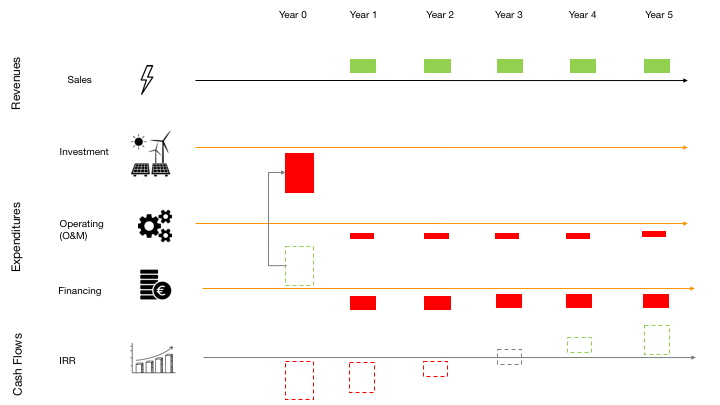
\includegraphics[width=1.00000\textwidth]{/Users/dvf/desktop/eba gitbook/Images/image7.png}
\caption{}
\end{figure}

The investment in the power plant has an initial investment that will be
done in year 0 (the present). We will be able to sell some electricity
back to the grid and for that we will have some positive cash flow from
sales, but there will be some operation and maintenance costs. We also
need to ask for a loan to develop the project, so we will have some
financing expenses throughout the years.

At the end, the balance between the investment, and the sales from power
plant minus the expenses in operating and financing will generate
sufficient cash flows not only to payback the investment in 3 years, but
also to generate additional earnings. Now, of course this depends on the
considered interest rate.

One important aspect in project evaluation is to look to the evolution
of cash flows and not only to the final end result (NPV, IRR or Payback
Period).

\subsection{Liquidity trap}\label{liquidity-trap}

The pitfall of just looking to NPV and not to cash flows or to answer
the simple question: will I have enough funds to pay all committed
obligations and?

Do I have working capital to secure is any future earning is delayed
lead companies to stressful situations. Using again the same
representation of Cash Flows and now imagine this planned cash flows.
All seem ok, there is enough money to pay O\&M, financing activities and
in year 5 IRR will be positive, meaning that you already repaid all
financial investment

Imagine you have a malfunction that had two consequences: a)Needed to
spend more money in O\&M and b) you were sole able to generate
electricity, so you will have no sales in this year. c)How are going to
pay for the financing activities?

This is the liquidity trap, when you may have a great balance sheet will
future revenues streams, but if you have few liquid resources for the
short run you may end in what is so called ``Financial Slack'' As a side
effect, even if you are able to borrow money, you IRR will also be worse
than forecasted and you will need to more time to have the expected
return on investment (that at this point you understand that also
carries a cost)

One of the most common traps is the liquidity trap than be framed as
follows:

What is worse? Owing 100\euro{} tomorrow or 1 \euro{} today?

Imagine company A that has 0\euro{} today but will receive 100\euro{}
tomorrow. The problem is if has to make payments today so, technically
could A)ask for a loan(which carries costs)

B)may be not able to secure such loan and technically would be bankrupt.

The pitfall of just looking to npv and not to cash flows or to answer
the simple question:will I have enough funds to pay all committed
obligations and? Do I have working capital to secure is any future
earning is delayed lead companies to stressful situations.This is the
liquidity trap, when you may have a great balance sheet will future
revenues streams,but if you have few liquid resources for the short run
you may end in what is so called ``Financial Slack''

This is called the liquidity trap, when your balance sheet with future
revenues streams looks good, but if you have few liquid resources for
the short run you may end by failing your duties. In this case, for
example, if you need to borrow additional money, you NPV will also be
worse than forecasted and you will need to more time to have the
expected return on investment. If you ha

You already understand cash flows still there are some details you
should consider: A Cash Flow is a stream of income (money) into or out
of a business, project, or financial product measured during a
specified, limited period of time. It corresponds to a stream of income,
where can change if you increase sales, or price or increase or decrease
costs, as savings.

So when looking do a cash flow statement,

We can see:

Revenues of Sales, or how much money in coming in,

Investment, meaning money spent on investments activities)

Operations, usually referred as Operations \& Maintenance (O\&M) and
Financing.

In green are all inflows of money, in red the outflows, so, breaking
down per year, a typical investment, demands high capital investment in
year 0 and if you don´t have, you may ask for a loan. So in year 0 you
have a loan that goes to investment activities. In year 1 you will have
inflows of money from sales, but you also have to pay for O\&M and
financing activities.

Lastly, if you notice, your IRR will go from a negative one to a
positive one. As you may notice, if don´t have enough inflows of cash to
pay for O\&M or Financing, you would end in a ``negative'' net cash flow
position, meaning that you are not generating enough income to pay for
your activities.

Coming back to the example of the PV System project, imagine that in
Year 3, there is a stop in the production. This has two consequences:
the money for Operation and Maintenance will increase, there will be no
sales, so we how are we going to pay for the financing activities?

\begin{figure}[htbp]
\centering
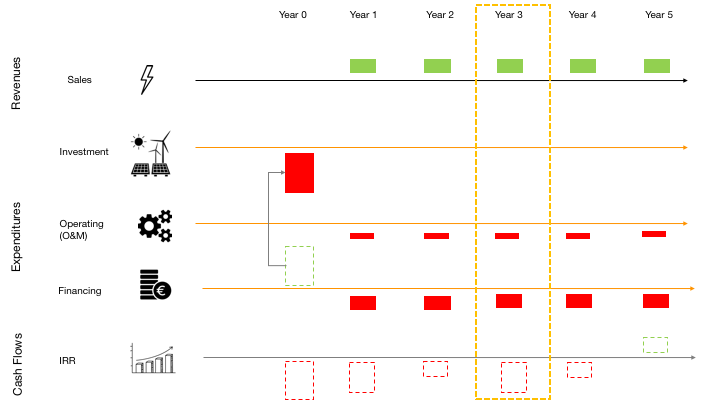
\includegraphics[width=1.00000\textwidth]{/Users/dvf/desktop/eba gitbook/Images/image8.png}
\caption{}
\end{figure}

\subsection{EE metrics}\label{ee-metrics}

\subsection{Levelized Cost of Energy
(LCOE)}\label{levelized-cost-of-energy-lcoe}

The LCOE Measures lifetime costs divided by energy production or:

• Calculates present value of the total cost of building and operating a
power plant over an assumed lifetime. • Allows the comparison of
different technologies (e.g., wind, solar, natural gas) of unequal life
spans, project size, different capital cost, risk, return, and
capacities

It is quite similar to the NPV formula, where:

\[LCOE = \sum_{t=1}^{n}\frac{I_t+M_t+F_t}{(1+r)^t}\]

It = Investment expenditures in year t (including financing) Mt =
Operations and maintenance expenditures in year t Ft = Fuel expenditures
in year t Et = Electricity generation in year t r = Discount rate n =
Life of the system Note on degrading factor

If the fuel also releases CO2 you also have to consider (if industrial)
the EU ETS Allowances (or other,depending on the countries regulation).

Focusing on the variable cost, the CO2 main price driver is the ``Fuel
Switching cost'' and coal forwards (coal releases more CO2) and gas
forwards, having a direct impact on power prices.

The price dynamic in the emissions market is driven by the power sector.

At the end, it gives a metric of the cost of energy by implementing the
projects, so the project with the lowest LCOE should in principle be
more advantageous.

For energy generation projects like PV Power plants, or energy savings
project (like changing the lighting system), the LCOE is quite similar
to the NPV formula and represents the ration between the stream of cash
Flows to generate the electricity (or saving electricity) during n years
divided by the energy produced (or consumed) during that period.

For example for the PV System project, where its have a 1 y term (for
simplicity), the LCOE would be:

\begin{figure}[htbp]
\centering
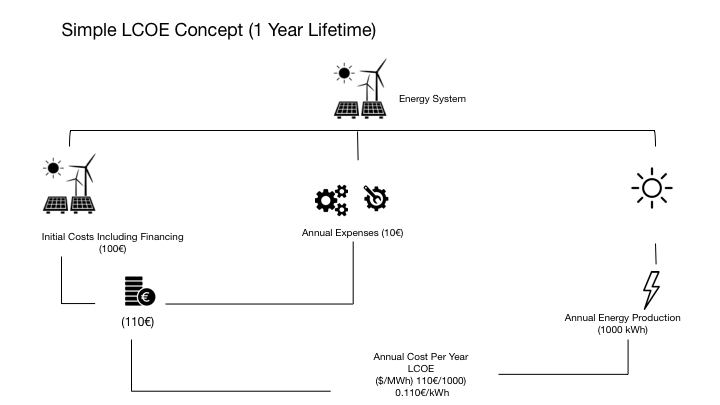
\includegraphics[width=1.00000\textwidth]{/Users/dvf/desktop/eba gitbook/Images/image9.png}
\caption{}
\end{figure}

The Initial Costs Including Financing (100\euro{}), plus Annual Expenses
(10\euro{}) (if you have more years, would be the projects O\&M), or
110\euro{} of costs.

Imagine that generates 1000kWh per year, so the costs of each would be
0.11\euro{}/kWh.

There are some things you should be aware when using this model:

\begin{itemize}
\tightlist
\item
  Increasing and decreasing the lifespan of equipment may change a lot
  results;
\item
  Efficiency of equipment tends to decrease over time and use (meaning
  that in year 10, you may not be able to generate the same amount of
  year 1)
\item
  If it relies on natural resources, you should be aware of
  intermittency of generation;
\item
  O\&M may increase due to overuse of equipment
\end{itemize}

\subsection{Cost-Optimaly Methodology}\label{cost-optimaly-methodology}

The Cost-Optimaly Methodology gives all relevant definitions needed to
make the cost-optimum calculations and analyses of the implementation of
energy efficiency measures in buildings.

It is defined as technologically neutral and does not favour one
technological solution over another. It ensures a competition of
measures/ packages/ variants over the estimated lifetime of a building
or building element''.

The global cost must be calculated according to EN15459 as indicated in
the formula:

\[C_{g}(\tau) = C_I \sum{_j}[ \sum_{i=1}^{\tau}(C_{a,i(j)} \cdot R_d(i)) - C_{f\tau}(j)]\]

Where:

Cg(t) are the Global costs referring to the starting year τ=0 Cl are the
Initial investment costs Ca,i(j) are the annual costs year i for
energy-related component j (energy costs, operational costs, periodic or
replacement costs, maintenance costs) Rd(i) is the discount rate for
year i (depending on interest rate) (minus) Vf,τ(j) is the final value
of component j at the end of the calculation period (referred to the
starting year τ=0 ).

The cost-optimum calculations are based on a net present value
calculation.

According to Boermans, Bettgenhäuser et al., 2011 ( Cost-optimal
building performance requirements - Calculation methodology to report on
national energy performance requirements on the basis of cost-optimality
within the framework of the EPBD, eceee).

when we discuss the cost-optimal levels and the effort to achieve energy
savings, only the lower boundary of the cloud is interesting to identify
the cost-optimal level. In case of a flat cost-curve, it was suggested
to set the requirements in the lower (left) part of the calculated
cost-optimal points. This will ensure that the most energy-efficient
solution sets are selected. On the other hand, one should also try to
avoid going too far on the left side of the curve, as cost-curves often
show a tendency of a steep increase in costs when moving to the far
left.

\begin{figure}[htbp]
\centering
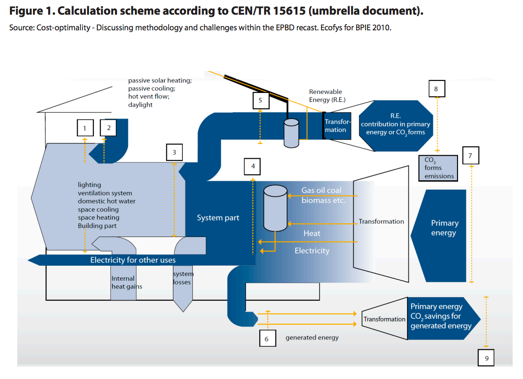
\includegraphics[width=1.00000\textwidth]{/Users/dvf/desktop/eba gitbook/Images/image10.png}
\caption{}
\end{figure}

Source
\url{http://bpie.eu/wp-content/uploads/2015/10/Implementing_Cost_Optimality.pdf}
pages 74 and 75

\section{Scenario and Risk Analysis}\label{scenario-and-risk-analysis}

\subsection{Risk and uncertainty}\label{risk-and-uncertainty}

When referring to risk, most relates to the idea if certainty (or the
lack of it) and or high or low volatility.

You understand that a deposit is safer than investing in the stock
market. For the last you will demand a higher return, or risk premium
(usually is equal to risk free rate plus a certain risk on top of that).
The later carries higher risk, that could mean you could lose all you
invested money (and more if you add some complex financial products).

\subsection{financial risk and operational
risk}\label{financial-risk-and-operational-risk}

It also refer to safety and reliability. In engineering usually it is
referred to risk as something you have to mitigate to guarantee a
certain level or safety, efficiency or other parameter or, to have safe
gauge in the case that something fails. As a control system that may
stop some task, send an alarm an so on.

So you have financial risk and operational risk, referring to the
implementation and operations of a certain investment.

Understanding risk, means understanding exposure, or what type of events
could change you basic underlying assumptions

\begin{itemize}
\tightlist
\item
  Technical and operational risk;
\item
  Regulatory risk;
\item
  Market Risk;
\item
  Financial Risk;
\end{itemize}

As an example if you run your projections assuming a certain amount of
sales and a small change will set to unprofitability, so running several
scenarios will help you understand how exposed you are to a change of
the demanded volume.

A change in regulation will set more companies working on the same space
so setting cannibalism behaviors (as dumping);

First you start by acknowledging the event, then mitigate or (trying to)
by different strategies. You may also choose to pursue option in less
probability to being exposed to a certain risk

One of the most common ones relies on technical and operational risk, or
how often projects access that the initial parameters still hold.

Basic example is can be described as follows:

Certain manufacturer states stat a certain equipment works for a
determined use and need repairs and maintenance every x year of other
parameter. Project managers wants to ``maximize profit and its being
working fine until now, nothing seems wrong'' so will save a few Euros
and delaying replacement of some fundamental pieces or maintenance and
looks great on the financial documents. Until a certain day where either
have a huge accident or the systems breaks.

It's the typical fat tail risk where from previous observations,
everything will look ``average''\ldots{} in historical data. If you
discard that some things will not decrease efficiency, just go from one
state to other, because reached a breaking point (or change of state).

Considering corporate finance, risk is priced ,usually by the Beta
Coefficient of the CAPM model, that coupons the minimum return adjusted
to risk

\subsection{Due diligence}\label{due-diligence}

Due diligence is verifying that all statements are true, this means
verifying all assumptions prior and then you should have proper
compliance mechanism to avoid having misrepresentation of the facts.

Projects are run by humans and humans (and machines) make errors, so you
always should have systems to track errors, not dependent in a single
person.

This is why you order audits to third parties which has 2 effects:
People will perform differently in they know someone else will
verifying;

If more than on person or entity will check the project, you will have
lower probability of missing some critical element or information.

Narrowed Due diligence so as corporate governance structure can mitigate
opportunist behaviors, misrepresentation of facts or important element
important to make any investment decision.

\subsection{Externalities}\label{externalities}

Finally, you can also consider other metrics, as environment impact (as
carbon footprint) and social impact in these projects.

So you also can incorporate on the initial goals so as quantifying such
metrics so as risks.

\subsection{Project evaluation steps}\label{project-evaluation-steps}

\begin{figure}[htbp]
\centering
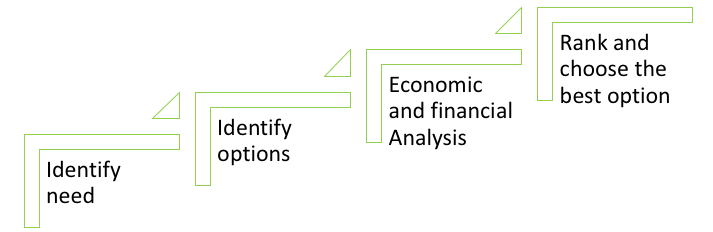
\includegraphics[width=1.00000\textwidth]{/Users/dvf/desktop/eba gitbook/Images/image11.png}
\caption{}
\end{figure}

Identify service need and define objectives and scope Identify options
to accomplish the objectives Narrow down the options Do the economic and
financial analysis of the different options Identify benefits (avoided
costs and saving costs) Identify investment and operation costs Evaluate
net benefits Due risk analysis and sensitivity analysis Rank and choose
the best option

\chapter{Energy Contracts}\label{energy-contracts}

\section{Basic Concepts}\label{basic-concepts-1}

When dealing with Energy Services, some of the main challenges are:

Challenges in energy efficiency - Most organizations (building owners)
don´t have the initial capital upfront to invest in Energy Efficiency
measures;

No capital for investment - Banks are not specialized in this type of
investment or, able to make an offer alone;

Difficulty to get bank loans - It´s a regulated market with technical
certification needed, so out of scope of the usual business of usual
lenders;

Technical complexity - Technical and complex deal structure, with
several entities; and

No standard contracts - The insistence of a real standard Contract
across countries or even within the same jurisdiction.

Most contracts are designed to answer a specific need or problem.

When we refer to a contract, on a very simples terms we mean:

An agreement with specific terms between two or more persons or entities
in which there is a promise to do something in return for a valuable
benefit (or consideration, in common law)

\begin{figure}[htbp]
\centering
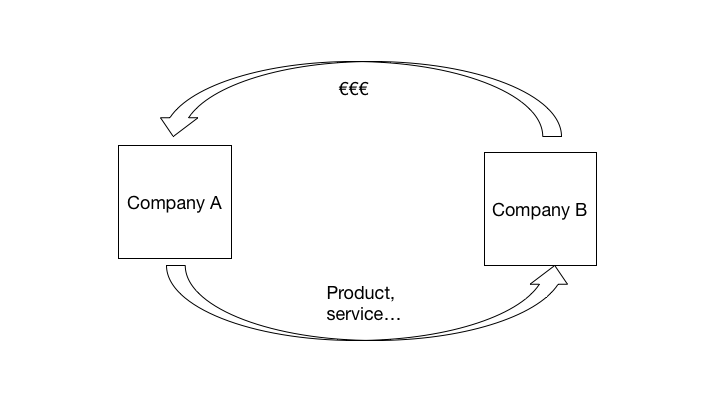
\includegraphics[width=1.00000\textwidth]{/Users/dvf/desktop/eba gitbook/Images/image31.png}
\caption{}
\end{figure}

The existence of a contract requires finding the following factual
elements:

an offer;

an acceptance of that offer which results in a meeting of the minds
(also referred as ``the mirror image rule'');

a promise to perform;

a valuable consideration (which can be a promise or payment in some
form);

a time or event when performance must be made (or also refereed as meet
commitments);

The terms and conditions for performance, including fulfilling promises;

performance, and

an intention to effect legal obligations (so we are excluding what
doctrine refers as ``not a serious proposal'' too)

Depending on how the deal is structured, performance and its payment can
be designed differently. Usually are dragged along the whole term of the
contract (not a single performance and payment), namely if there are
several installments instead of a single payment or, it´s a recurrent
service.

Contract elements

Performance and Payment

Exhange (product /service) for a

Price

Terms and conditions

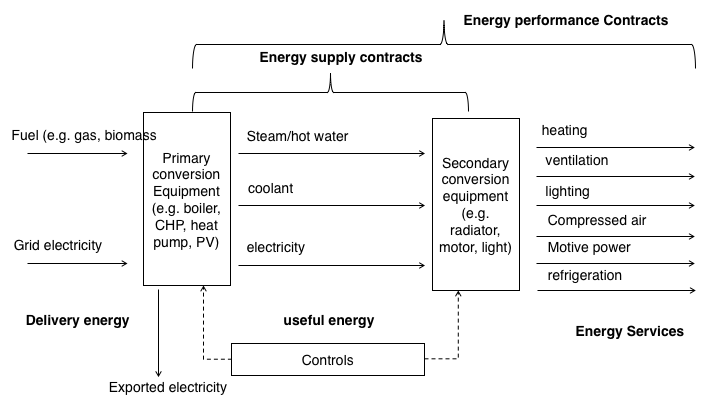
\includegraphics[width=1.00000\textwidth]{/Users/dvf/desktop/eba gitbook/Images/image32.png}
The total energy used (not useful) can be expressed as how we use energy
services, or secondary conversation that concerts to heating,
ventilation, lighting and so on.

Bear in mind, that energy supply and energy performance are not
equivalents. Contracting a certain amount of energy and an end use are
not equals. Besides losses with secondary conversion, the first is
related to a commodity (or raw material you buy to generated a certain
output), the last to the end result.

The same amount of energy may give the same thermal comfort, or not, for
example.

Energy contracts:

Energy Supply Contracts

Power Purchase Agreements (PPAs)

Energy Services Agreement (ESAs)

Energy Management Contracts (EMCs)

Energy Performance Contracts (EPCs)

Finally, to have a Contract you need, at least two persons or entities.

The Energy Efficiency Directive (EED) defines an `energy service
provider' as a ``natural or legal person who delivers energy services or
other energy efficiency improvement measures in a final customer's
facility or premises''.

They can be (alone or jointly):

-Utilities;

-Equipment manufacture/supplier;

-Supplier Manufacturer of building automation and control systems

-Facility management and operation company

-Consulting/engineering firm

-Independent specialist (focused on Energy efficiency services);

-Energy Data Companies;

-Governmental entities (namely under subsidized schemes)

-Banks and other Financial institutions (as intermediaries for EE
related type of investments) and

-Others.

In a raw sense, you should understand that entity will not define the
contract, meaning that a EPC will be a EPC, regardless if is specially
used by one type of Entity (typical example of EE contracts with the
Public Sector). Also, you can have a variety of entities so
understanding the responsibility, strengths and weaknesses and
governance among them is an import matter.

Finally, To have a Contract you need, at least two persons or entities.

The Energy Efficiency Directive (EED) defines an `energy service
provider' as a ``natural or legal person who delivers energy services or
other energy efficiency improvement measures in a final customer's
facility or premises''.

\section{PPA´s}\label{ppas}

A power purchase agreement (PPA), or electricity power agreement, is a
contract between two parties, one which generates electricity (the
seller) and one which is looking to purchase electricity (the buyer).
The PPA defines all of the commercial terms for the sale of electricity
- it can be fixed, indexed or ``shaped''- between the two parties,
including when the project will begin commercial operation, schedule for
delivery of electricity, penalties for under delivery, payment terms,
and termination. A PPA is the principal agreement that defines the
revenue and credit quality of a generating project and is thus a key
instrument of project finance.

This differs from the traditional approach of simply buying electricity
from licensed electricity suppliers, often known as utility (or
wholesale) PPAs. PPA also are a way of choosing a certain type of
energy, the most common example, if a company wants to achieved a
certain percentage of renewables (or decrease its carbon footprint) to
either improve overall rating of its assets (from real estate to overall
company), doing a PPA with solar or wind farm is a way to achieve that
goal.

There are several Business Models Involving PPAs We can have:

On-site sale

-- Direct sale to customer on site (shopping centres, commercial
centres, manufacturing industry, airports, ports etc.)

-- Saves costs related to the use of the transmission grid
(transmission, distribution, dispatching, general costs of system)

Or Sale through the grid

-- Utility scale ground-mounted plants;

-- Sale to energy utilities (peak load purchases, renewable energy
source obligations);

-- Sale to end users (large industrial clients);

-- Sale to wholesalers or ``aggregators'';

There are several Power Purchase Agreement structures, namely:

Onsite direct wire PPA

Sleeved off-site PPA

Synthetic PPA

Mini-utility

Wholesale PPA

\begin{figure}[htbp]
\centering
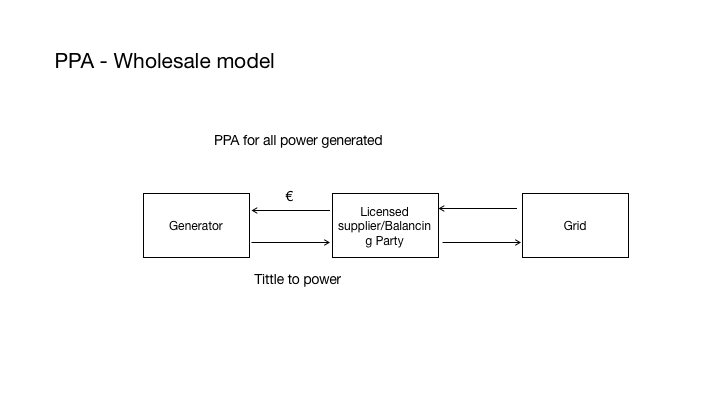
\includegraphics[width=1.00000\textwidth]{/Users/dvf/desktop/eba gitbook/Images/image33.png}
\caption{}
\end{figure}

The most simple PPA is the ``Wholesale model'', where the generator
sells all power supplier back to the grid. Most of the RES where
implemented using this structure, where licenses where auctioned to
generate a certain amount of energy in an exchange for a certain
predefined tariff per MWh.

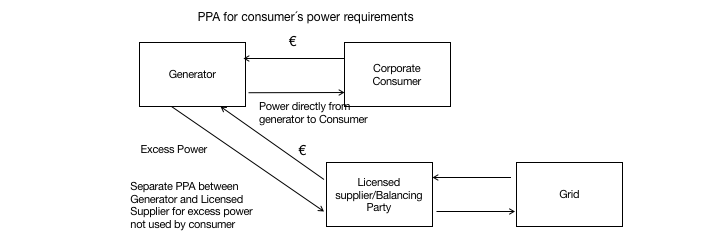
\includegraphics[width=1.00000\textwidth]{/Users/dvf/desktop/eba gitbook/Images/image34.png}
Not all PPA are wholesale PPA´s and increasingly we see more often
onsite private wire PPA´s. Instead of selling all back to the grid,
namely activities that are energy intensive, as running servers of a
company, or, they want to improve the \% of RES in their overall energy
mix, they can have power directly from generator to them and, a separate
PPA, for either the excess power produced or as a last resort supplier.

\begin{figure}[htbp]
\centering
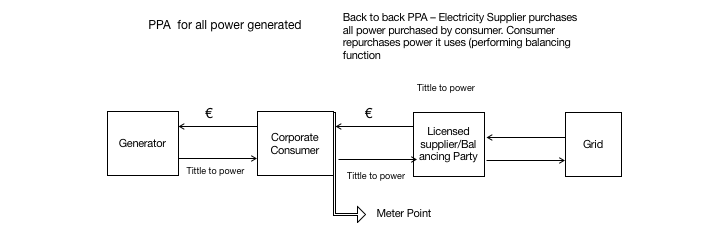
\includegraphics[width=1.00000\textwidth]{/Users/dvf/desktop/eba gitbook/Images/image35.png}
\caption{}
\end{figure}

In a Sleeved PPA, all power generated is sold by the corporate consumer
to the licensed supplier -- or balancing party -- still is a Back to
back PPA -- Electricity Supplier purchases all power purchased by
consumer. Consumer repurchases power it uses (performing balancing
function).

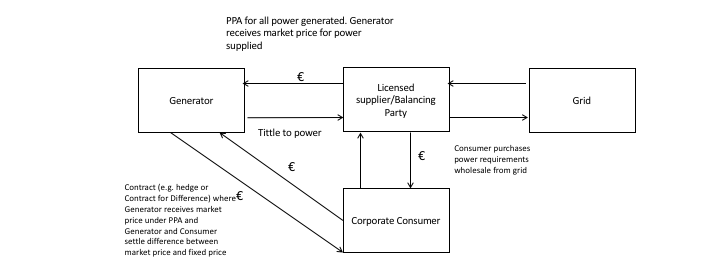
\includegraphics[width=1.00000\textwidth]{/Users/dvf/desktop/eba gitbook/Images/image36.png}
A Synthetic PPA or, also referred as a ``Virtual PPA'' is a Contract
(e.g.~hedge or Contract for Difference) where Generator receives market
price under PPA and Generator and Consumer settle difference between
market price and fixed price. Its virtual, because there is no physical
purchased of electricity, like most Contract for Difference. If you
already looked to commodities trading (as brent, for example), you you
see that most have ``financial liquidation and not physical liquidation.

\begin{figure}[htbp]
\centering
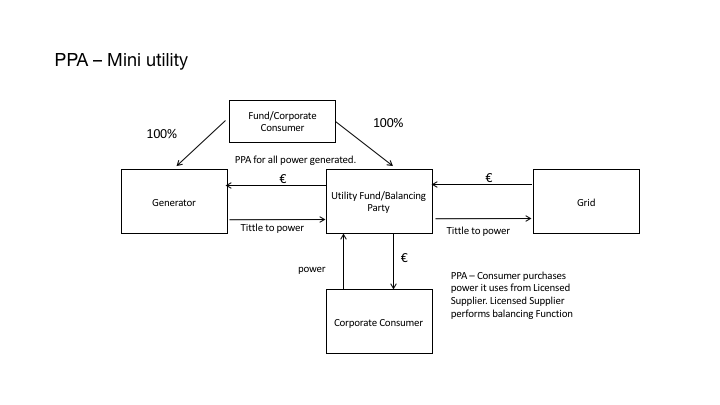
\includegraphics[width=1.00000\textwidth]{/Users/dvf/desktop/eba gitbook/Images/image37.png}
\caption{}
\end{figure}

Lastly, a mini utility PPA -- Consumer purchases power it uses from
Licensed Supplier. Licensed Supplier performs balancing Function too.

\subsection{Curtailments}\label{curtailments}

There are what so called Default provisions related to Curtailments

\begin{figure}[htbp]
\centering
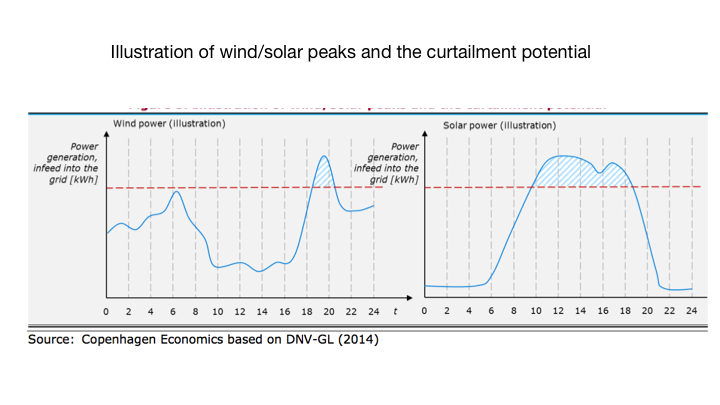
\includegraphics[width=1.00000\textwidth]{/Users/dvf/desktop/eba gitbook/Images/image38.png}
\caption{}
\end{figure}

On the Buyer-Directed Curtailment: -- Buyer may have the right to direct
Seller to decrease or stop deliveries -- Generally for economic reasons
-- Seller should be compensated -- Make sure the Project is capable of
complying

Third-Party Curtailment: -- Interconnecting Utility or Transmission
Provider -- Broad curtailment rights in Interconnection Agreement --
e.g.~emergency, reliability, system maintenance -- Frequency may depend
on level of transmission service -- Seller may or may not be compensated

Curtailments can be Compensated or not, where:

On the Compensated Curtailments: -- Contract Price for each MWh Seller
could have delivered -- Plus, if applicable, value of lost benefits,
grossed up for taxes

Or Non-Compensated Curtailments: -- Big negotiation point and financing
issue -- Seller wants to maximize ability to get compensated -- argument
is that anything affecting transmission beyond the the Point of Delivery
(POD) is Buyer's risk -- Generally no compensation for an ``Emergency''
-- Buyer treats this like a force majeure; definition is important --
Generally no compensation if curtailment results from Seller's failure
to maintain required permits or interconnection facilities at or prior
to the Point of Delivery (POD) -- Mechanics depend on market rules and
Project specifics -- Be careful if Buyer is also the Transmission
Provider or Interconnecting Utility

\section{Incentives and other schemes to support EE
implementation}\label{incentives-and-other-schemes-to-support-ee-implementation}

The Article 18 of the EED (Energy Efficiency Directive) stablishes
regarding ``Energy services'', that all Member States shall promote
Energy Services and access by disseminating clear and easily accessible
information, among other; on: (i) available energy service contracts and
clauses that should be included in such contracts to guarantee energy
savings and final customers' rights; (ii) financial instruments,
incentives, grants and loans to support energy efficiency service
projects; (i) providing model contracts for energy performance
contracting which include at least the items listed in Annex XIII;

Direct support as:

-Grants/Subsidies that can be as: Subsidy on a certain percentage of EE
investment (CAPEX); or Financial Mechanism (Loans, Credit
line\ldots{})., with better finantial terms as offereced by usual
lenders, as banks. Most of the times, banks offered this termsunder
certain governmental initiative, so they act as intermediaties of such
Financial mechanims too.

Or as a Fiscal incentives, such as Rebates Deductions over taxable
income (\ldots{}) Or other schemes

They can be:

Special Purpose Vehicle (SPV), or a legal person, a company to perform a
certain task/goal, Direct loan to acquire equipment + services contract;
Rental with buy option (leasing); Other;

The main implications and differences may are: ownership and risk
(namely in some events such as: bankruptcy, breach of contract, etc)

Lastly there are EE targets for specific sectors, namely for

\begin{verbatim}
non SME´s, 
Specific industries (large combustion plants), 
Energy intense activities;
Public sector, etc)
\end{verbatim}

There are targets these type of entities must comply under the general
EED or other national legislation. Unlike the other cases, were such
improvements are not mandatory, this entities have a strong incentive:
legal one, not a market one.

\subsection{Interconnections with Public
Law}\label{interconnections-with-public-law}

Most of the EE contracts may fall into a Public Contract (namely if you
managing a public building, as a public hospital, school):

A Public Contract (also referred as Public Procurement) can be defined
by Subjective or objective imputation, as:

\begin{itemize}
\tightlist
\item
  By type or entity (Public Entities and related);
\item
  By type of Contract (more than 50\% financed by public funds);
\end{itemize}

By sectorial areas (specific utilities markets in certain countries may
be exempt from public procurement rules): If you will be considering
using national or EU financial schemes you may have to fulfill public
procurement rules, even not being a public entity, but because more than
than 50\% is financed by public funds)

For a utilities market to be exempt: the legal/regulatory environment
permits access and competition in the sector concerned; the utility
operators in the market concerned are subject to competitive pressure.

The are Thresholds

EU law sets minimum harmonised rules for tenders whose monetary value
exceeds a certain amount and which are presumed to be of cross-border
interest. The European rules ensure that the award of contracts of
higher value for the provision of public goods and services must be
fair, equitable, transparent and non-discriminatory. For tenders of
lower value however, national rules apply, which nevertheless must
respect general principles of EU law.

\chapter{Conclusion}\label{conclusion}

\section{Main insights}\label{main-insights}

VC investment in Portugal relies, mostly on public funds with an absence
of evidence of return of investment adjusted to risk.

Comparing, there are few ``high growth companies'' and they seem to be
in economic areas different that the invested ones. Unlike the idea that
all VC deals are different, data show that same degree and forms of
investments are used, not in equity instruments, rather in debt
instruments. The use of typical instruments of public liability company,
as securities are not used, besides issuance of shares.

There is also no evidence that the change on share capital requirement
created a significant change in the number of companies.

In spite of a lot of promotion of ``startups'', results are yet to be
demonstrated.

The last of buy side also seems to be a contact, where exists are mostly
trough outside countries. The concentration of the market share in few
players (most being public funded) also contracts with an idea of market
based, but rather policy based. Incentives are drawn by regulation (and
funding of State), not market.

The rolling of this assets seems also to be an issue, where no cash (as
a fungible and more liquid asset) seems to be realized, rather selling
stats to other funds, for reimbursement of the first.

Most observations are not even distributed, meaning that a small
percentage have a higher weight than the most frequent ones. It´s a
typical case of extreme value distributions, with highly skewed
distributions.

\section{According to available data, account should be
taken:}\label{according-to-available-data-account-should-be-taken}

\begin{enumerate}
\def\labelenumi{\alph{enumi})}
\item
  No IPO's (between the period 2007 to 2015 there are 0 occurrences of
  this form of disinvestment), even considering the total capital
  (venture capital and private equity), being able to conclude that
  there is a weak depth of Capital markets;
\item
  The Government (directly and indirectly) as one of the major players,
  where in the investment policy is visible the limitations on the
  instruments used, as well as on the location and investment area. It
  can be stated that the investment, is in line with structural support
  funds (Compe case, QREN and currently P2020).
\end{enumerate}

\subsection{Future work}\label{future-work}

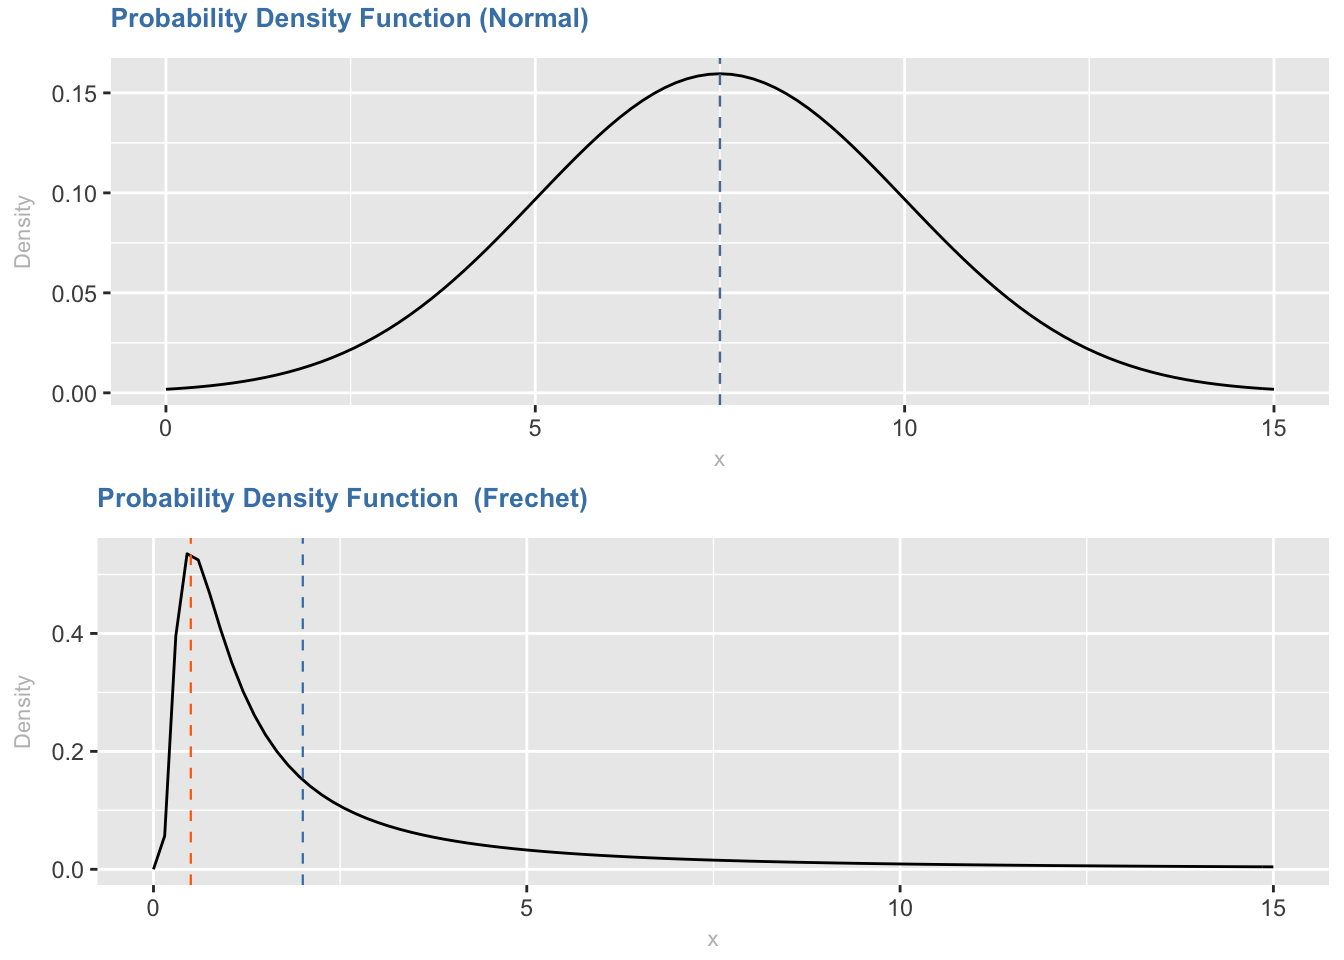
\includegraphics{EBA_Notes_files/figure-latex/unnamed-chunk-4-1.pdf}

\chapter{Annexes}\label{annexes}

Notes

Portugal Ventures

There were several inconsistencies between the Funds reports from 2012
to 2015 (latest available), particularly in assets under management.

Taking into consideration the merger, extinction and spin-off of several
funds, it is important to take into account that, according to data from
Portugal Ventures, it manages ``Funds under management: (approximately)
\euro{} 400 million.'' (Turismo de Portugal, FAI and some of the AICEP),
but this is a management entity and has a double criterion in reports
that, on the one hand, it reports (in particular to assess the capital
gains of FAI Energia), but it is completely omitted and does not, in
fact, include all the assets under management.

TABLE

\begin{longtable}[]{@{}llll@{}}
\toprule
\begin{minipage}[b]{0.17\columnwidth}\raggedright\strut
Type\strut
\end{minipage} & \begin{minipage}[b]{0.17\columnwidth}\raggedright\strut
Incorporation\strut
\end{minipage} & \begin{minipage}[b]{0.17\columnwidth}\raggedright\strut
Change\strut
\end{minipage} & \begin{minipage}[b]{0.17\columnwidth}\raggedright\strut
Holding, stage\strut
\end{minipage}\tabularnewline
\midrule
\endhead
\begin{minipage}[t]{0.17\columnwidth}\raggedright\strut
1\strut
\end{minipage} & \begin{minipage}[t]{0.17\columnwidth}\raggedright\strut
FCR PORTUGAL VENTURES VALOR\strut
\end{minipage} & \begin{minipage}[t]{0.17\columnwidth}\raggedright\strut
20-07-1994\strut
\end{minipage} & \begin{minipage}[t]{0.17\columnwidth}\raggedright\strut
15-12-2014\strut
\end{minipage}\tabularnewline
\begin{minipage}[t]{0.17\columnwidth}\raggedright\strut
2\strut
\end{minipage} & \begin{minipage}[t]{0.17\columnwidth}\raggedright\strut
FCR PORTUGAL VENTURES\strut
\end{minipage} & \begin{minipage}[t]{0.17\columnwidth}\raggedright\strut
19-01-1993\strut
\end{minipage} & \begin{minipage}[t]{0.17\columnwidth}\raggedright\strut
15-12-2014\strut
\end{minipage}\tabularnewline
\begin{minipage}[t]{0.17\columnwidth}\raggedright\strut
3\strut
\end{minipage} & \begin{minipage}[t]{0.17\columnwidth}\raggedright\strut
FCR PORTUGAL VENTURES GLOBAL\strut
\end{minipage} & \begin{minipage}[t]{0.17\columnwidth}\raggedright\strut
01-06-1999\strut
\end{minipage} & \begin{minipage}[t]{0.17\columnwidth}\raggedright\strut
01-12-2013\strut
\end{minipage}\tabularnewline
\begin{minipage}[t]{0.17\columnwidth}\raggedright\strut
4\strut
\end{minipage} & \begin{minipage}[t]{0.17\columnwidth}\raggedright\strut
FCR PORTUGAL VENTURES INTER-REGIONAL\strut
\end{minipage} & \begin{minipage}[t]{0.17\columnwidth}\raggedright\strut
21-12-1999\strut
\end{minipage} & \begin{minipage}[t]{0.17\columnwidth}\raggedright\strut
31-12-2014\strut
\end{minipage}\tabularnewline
\begin{minipage}[t]{0.17\columnwidth}\raggedright\strut
5\strut
\end{minipage} & \begin{minipage}[t]{0.17\columnwidth}\raggedright\strut
FCR PORTUGAL VENTURES VALOR 2\strut
\end{minipage} & \begin{minipage}[t]{0.17\columnwidth}\raggedright\strut
11-08-1994\strut
\end{minipage}\tabularnewline
\begin{minipage}[t]{0.17\columnwidth}\raggedright\strut
6\strut
\end{minipage} & \begin{minipage}[t]{0.17\columnwidth}\raggedright\strut
FCR PORTUGAL VENTURES 2\strut
\end{minipage} & \begin{minipage}[t]{0.17\columnwidth}\raggedright\strut
28-01-1993\strut
\end{minipage} & \begin{minipage}[t]{0.17\columnwidth}\raggedright\strut
01-12-2013\strut
\end{minipage}\tabularnewline
\begin{minipage}[t]{0.17\columnwidth}\raggedright\strut
7\strut
\end{minipage} & \begin{minipage}[t]{0.17\columnwidth}\raggedright\strut
FCR PORTUGAL VENTURES TIEC\strut
\end{minipage} & \begin{minipage}[t]{0.17\columnwidth}\raggedright\strut
06-03-1998\strut
\end{minipage} & \begin{minipage}[t]{0.17\columnwidth}\raggedright\strut
01-12-2013\strut
\end{minipage}\tabularnewline
\begin{minipage}[t]{0.17\columnwidth}\raggedright\strut
8\strut
\end{minipage} & \begin{minipage}[t]{0.17\columnwidth}\raggedright\strut
FCR PORTUGAL VENTURES GLOBAL 2\strut
\end{minipage} & \begin{minipage}[t]{0.17\columnwidth}\raggedright\strut
15-07-1999\strut
\end{minipage}\tabularnewline
\begin{minipage}[t]{0.17\columnwidth}\raggedright\strut
9\strut
\end{minipage} & \begin{minipage}[t]{0.17\columnwidth}\raggedright\strut
FCR PORTUGAL VENTURES TURISMO\strut
\end{minipage} & \begin{minipage}[t]{0.17\columnwidth}\raggedright\strut
25-08-1995\strut
\end{minipage} & \begin{minipage}[t]{0.17\columnwidth}\raggedright\strut
TC (not reported)\strut
\end{minipage}\tabularnewline
\begin{minipage}[t]{0.17\columnwidth}\raggedright\strut
10\strut
\end{minipage} & \begin{minipage}[t]{0.17\columnwidth}\raggedright\strut
FCR PORTUGAL VENTURES GRANDES PROJECTOS DE INVESTIMENTO\strut
\end{minipage} & \begin{minipage}[t]{0.17\columnwidth}\raggedright\strut
09-08-2004\strut
\end{minipage} & \begin{minipage}[t]{0.17\columnwidth}\raggedright\strut
AICEP\strut
\end{minipage}\tabularnewline
\begin{minipage}[t]{0.17\columnwidth}\raggedright\strut
11\strut
\end{minipage} & \begin{minipage}[t]{0.17\columnwidth}\raggedright\strut
FCR PORTUGAL VENTURES - FIEP\strut
\end{minipage} & \begin{minipage}[t]{0.17\columnwidth}\raggedright\strut
29-12-2004\strut
\end{minipage} & \begin{minipage}[t]{0.17\columnwidth}\raggedright\strut
AICEP (not reported)\strut
\end{minipage}\tabularnewline
\begin{minipage}[t]{0.17\columnwidth}\raggedright\strut
12\strut
\end{minipage} & \begin{minipage}[t]{0.17\columnwidth}\raggedright\strut
FCR PORTUGAL VENTURES FINICIA\strut
\end{minipage} & \begin{minipage}[t]{0.17\columnwidth}\raggedright\strut
04-05-2007\strut
\end{minipage}\tabularnewline
\begin{minipage}[t]{0.17\columnwidth}\raggedright\strut
13\strut
\end{minipage} & \begin{minipage}[t]{0.17\columnwidth}\raggedright\strut
FCR FAI PORTUGAL VENTURES ENERGIAS\strut
\end{minipage} & \begin{minipage}[t]{0.17\columnwidth}\raggedright\strut
06-05-2009\strut
\end{minipage} & \begin{minipage}[t]{0.17\columnwidth}\raggedright\strut
FAI (not reported)\strut
\end{minipage}\tabularnewline
\begin{minipage}[t]{0.17\columnwidth}\raggedright\strut
14\strut
\end{minipage} & \begin{minipage}[t]{0.17\columnwidth}\raggedright\strut
FCR PORTUGAL VENTURES ACELERADOR DE COMERCIALIZAÇÃO DE TECNOLOGIAS\strut
\end{minipage} & \begin{minipage}[t]{0.17\columnwidth}\raggedright\strut
24-08-2009\strut
\end{minipage} & \begin{minipage}[t]{0.17\columnwidth}\raggedright\strut
31-12-2014\strut
\end{minipage}\tabularnewline
\begin{minipage}[t]{0.17\columnwidth}\raggedright\strut
15\strut
\end{minipage} & \begin{minipage}[t]{0.17\columnwidth}\raggedright\strut
FCR PORTUGAL VENTURES FIAEA - FUNDO DE INVESTIMENTO DE APOIO AO
EMPREENDEDORISMO DOS AÇORES\strut
\end{minipage} & \begin{minipage}[t]{0.17\columnwidth}\raggedright\strut
14-01-2011\strut
\end{minipage}\tabularnewline
\begin{minipage}[t]{0.17\columnwidth}\raggedright\strut
16\strut
\end{minipage} & \begin{minipage}[t]{0.17\columnwidth}\raggedright\strut
FCR PORTUGAL VENTURES BIOCANT\strut
\end{minipage} & \begin{minipage}[t]{0.17\columnwidth}\raggedright\strut
28-12-2011\strut
\end{minipage}\tabularnewline
\begin{minipage}[t]{0.17\columnwidth}\raggedright\strut
17\strut
\end{minipage} & \begin{minipage}[t]{0.17\columnwidth}\raggedright\strut
FCR PORTUGAL INTERNACIONALIZAÇÃO\strut
\end{minipage} & \begin{minipage}[t]{0.17\columnwidth}\raggedright\strut
18-04-2011\strut
\end{minipage} & \begin{minipage}[t]{0.17\columnwidth}\raggedright\strut
AICEP (reported)\strut
\end{minipage}\tabularnewline
\begin{minipage}[t]{0.17\columnwidth}\raggedright\strut
18\strut
\end{minipage} & \begin{minipage}[t]{0.17\columnwidth}\raggedright\strut
FCR PORTUGAL VENTURES INDUSTRIAS CRIATIVAS 01-09-2011\strut
\end{minipage}\tabularnewline
\begin{minipage}[t]{0.17\columnwidth}\raggedright\strut
19\strut
\end{minipage} & \begin{minipage}[t]{0.17\columnwidth}\raggedright\strut
FCR PORTUGAL VENTURES EARLY STAGE\strut
\end{minipage} & \begin{minipage}[t]{0.17\columnwidth}\raggedright\strut
30-09-2011\strut
\end{minipage}\tabularnewline
\begin{minipage}[t]{0.17\columnwidth}\raggedright\strut
20\strut
\end{minipage} & \begin{minipage}[t]{0.17\columnwidth}\raggedright\strut
FCR PORTUGAL VENTURES UNIVERSITAS\strut
\end{minipage} & \begin{minipage}[t]{0.17\columnwidth}\raggedright\strut
28-12-2011\strut
\end{minipage}\tabularnewline
\begin{minipage}[t]{0.17\columnwidth}\raggedright\strut
21\strut
\end{minipage} & \begin{minipage}[t]{0.17\columnwidth}\raggedright\strut
FCR PORTUGAL VENTURES ACELERADOR DE COMERCIALIZAÇÃO DE TECNOLOGIA
II\strut
\end{minipage} & \begin{minipage}[t]{0.17\columnwidth}\raggedright\strut
18-11-2011\strut
\end{minipage}\tabularnewline
\begin{minipage}[t]{0.17\columnwidth}\raggedright\strut
22\strut
\end{minipage} & \begin{minipage}[t]{0.17\columnwidth}\raggedright\strut
FCR PORTUGAL GLOBAL VENTURES I\strut
\end{minipage} & \begin{minipage}[t]{0.17\columnwidth}\raggedright\strut
17-06-2015\strut
\end{minipage}\tabularnewline
\begin{minipage}[t]{0.17\columnwidth}\raggedright\strut
23\strut
\end{minipage} & \begin{minipage}[t]{0.17\columnwidth}\raggedright\strut
FCR DINAMIZAÇÃO TURISMO\strut
\end{minipage} & \begin{minipage}[t]{0.17\columnwidth}\raggedright\strut
TC (not reported)\strut
\end{minipage}\tabularnewline
\begin{minipage}[t]{0.17\columnwidth}\raggedright\strut
24\strut
\end{minipage} & \begin{minipage}[t]{0.17\columnwidth}\raggedright\strut
FCR TURISMO - INOVAÇÃO\strut
\end{minipage} & \begin{minipage}[t]{0.17\columnwidth}\raggedright\strut
TC\strut
\end{minipage} & \begin{minipage}[t]{0.17\columnwidth}\raggedright\strut
(not reported, there are operations through this funds)\strut
\end{minipage}\tabularnewline
\begin{minipage}[t]{0.17\columnwidth}\raggedright\strut
25\strut
\end{minipage} & \begin{minipage}[t]{0.17\columnwidth}\raggedright\strut
FCR GLOBAL III\strut
\end{minipage} & \begin{minipage}[t]{0.17\columnwidth}\raggedright\strut
AICEP (not reported)\strut
\end{minipage}\tabularnewline
\begin{minipage}[t]{0.17\columnwidth}\raggedright\strut
26\strut
\end{minipage} & \begin{minipage}[t]{0.17\columnwidth}\raggedright\strut
FCR PORTUGAL VENTURES II\strut
\end{minipage} & \begin{minipage}[t]{0.17\columnwidth}\raggedright\strut
AICEP\strut
\end{minipage} & \begin{minipage}[t]{0.17\columnwidth}\raggedright\strut
(not reported) dissolution\strut
\end{minipage}\tabularnewline
\begin{minipage}[t]{0.17\columnwidth}\raggedright\strut
9\strut
\end{minipage} & \begin{minipage}[t]{0.17\columnwidth}\raggedright\strut
Incorporation\strut
\end{minipage} & \begin{minipage}[t]{0.17\columnwidth}\raggedright\strut
(+1)\strut
\end{minipage} & \begin{minipage}[t]{0.17\columnwidth}\raggedright\strut
Total in activity\strut
\end{minipage}\tabularnewline
\bottomrule
\end{longtable}

On the other hand, it does not report its position or affiliated
entities to the Directorate-General for the Treasury and Finance
{[}\^{}59{]} (there are only the management reports of the date of their
incorporation), where the changes are known, in particular as part of
the restructuring operation in 2012, in which 2014 had more changes and
from 2014 to 2015 there is an asset rotation that is not explained.

{[}\^{}59{]} : Report of the State Business Sector Entities, should be
present and available at:
\url{http://www.dgtf.pt/centro-de-documentacao-e-legislacao?tabid=993}

The reconstruction (possible, taking into account the constantly
changing amounts in portfolios and occurred changes due to mergers):

\begin{longtable}[]{@{}lllll@{}}
\toprule
\begin{minipage}[b]{0.17\columnwidth}\raggedright\strut
2011\strut
\end{minipage} & \begin{minipage}[b]{0.17\columnwidth}\raggedright\strut
2012\strut
\end{minipage} & \begin{minipage}[b]{0.17\columnwidth}\raggedright\strut
2013\strut
\end{minipage} & \begin{minipage}[b]{0.17\columnwidth}\raggedright\strut
2014\strut
\end{minipage} & \begin{minipage}[b]{0.17\columnwidth}\raggedright\strut
2015\strut
\end{minipage}\tabularnewline
\midrule
\endhead
\begin{minipage}[t]{0.17\columnwidth}\raggedright\strut
1.Total Subscribed Net Investment\strut
\end{minipage} & \begin{minipage}[t]{0.17\columnwidth}\raggedright\strut
310.8\strut
\end{minipage} & \begin{minipage}[t]{0.17\columnwidth}\raggedright\strut
203.6\strut
\end{minipage} & \begin{minipage}[t]{0.17\columnwidth}\raggedright\strut
198.5\strut
\end{minipage} & \begin{minipage}[t]{0.17\columnwidth}\raggedright\strut
201.1\strut
\end{minipage}\tabularnewline
\begin{minipage}[t]{0.17\columnwidth}\raggedright\strut
(Share capital entities - Shareholdings)\strut
\end{minipage} & \begin{minipage}[t]{0.17\columnwidth}\raggedright\strut
\strut
\end{minipage} & \begin{minipage}[t]{0.17\columnwidth}\raggedright\strut
\strut
\end{minipage} & \begin{minipage}[t]{0.17\columnwidth}\raggedright\strut
\strut
\end{minipage} & \begin{minipage}[t]{0.17\columnwidth}\raggedright\strut
\strut
\end{minipage}\tabularnewline
\begin{minipage}[t]{0.17\columnwidth}\raggedright\strut
1.Direct interests (holdings)\strut
\end{minipage} & \begin{minipage}[t]{0.17\columnwidth}\raggedright\strut
344\strut
\end{minipage} & \begin{minipage}[t]{0.17\columnwidth}\raggedright\strut
334\strut
\end{minipage} & \begin{minipage}[t]{0.17\columnwidth}\raggedright\strut
295.5\strut
\end{minipage} & \begin{minipage}[t]{0.17\columnwidth}\raggedright\strut
257.49\strut
\end{minipage}\tabularnewline
\begin{minipage}[t]{0.17\columnwidth}\raggedright\strut
1.1 In companies\strut
\end{minipage} & \begin{minipage}[t]{0.17\columnwidth}\raggedright\strut
17.6\strut
\end{minipage} & \begin{minipage}[t]{0.17\columnwidth}\raggedright\strut
14.4\strut
\end{minipage} & \begin{minipage}[t]{0.17\columnwidth}\raggedright\strut
4.6\strut
\end{minipage} & \begin{minipage}[t]{0.17\columnwidth}\raggedright\strut
30.3*\strut
\end{minipage}\tabularnewline
\begin{minipage}[t]{0.17\columnwidth}\raggedright\strut
1.2 In Funds\strut
\end{minipage} & \begin{minipage}[t]{0.17\columnwidth}\raggedright\strut
31.9\strut
\end{minipage} & \begin{minipage}[t]{0.17\columnwidth}\raggedright\strut
22.2\strut
\end{minipage} & \begin{minipage}[t]{0.17\columnwidth}\raggedright\strut
22.6\strut
\end{minipage} & \begin{minipage}[t]{0.17\columnwidth}\raggedright\strut
23.7\strut
\end{minipage}\tabularnewline
\begin{minipage}[t]{0.17\columnwidth}\raggedright\strut
2. Indirect interests\strut
\end{minipage} & \begin{minipage}[t]{0.17\columnwidth}\raggedright\strut
308.8\strut
\end{minipage} & \begin{minipage}[t]{0.17\columnwidth}\raggedright\strut
308.1\strut
\end{minipage} & \begin{minipage}[t]{0.17\columnwidth}\raggedright\strut
275.71\strut
\end{minipage} & \begin{minipage}[t]{0.17\columnwidth}\raggedright\strut
227.49\strut
\end{minipage}\tabularnewline
\begin{minipage}[t]{0.17\columnwidth}\raggedright\strut
2.2 Share Capital of entities (companies´holdings )\strut
\end{minipage} & \begin{minipage}[t]{0.17\columnwidth}\raggedright\strut
247.4\strut
\end{minipage} & \begin{minipage}[t]{0.17\columnwidth}\raggedright\strut
131.19\strut
\end{minipage} & \begin{minipage}[t]{0.17\columnwidth}\raggedright\strut
74.15\strut
\end{minipage} & \begin{minipage}[t]{0.17\columnwidth}\raggedright\strut
30.3*\strut
\end{minipage}\tabularnewline
\begin{minipage}[t]{0.17\columnwidth}\raggedright\strut
2.2 Share Capital of entities under management (Funds)\strut
\end{minipage} & \begin{minipage}[t]{0.17\columnwidth}\raggedright\strut
183.6\strut
\end{minipage} & \begin{minipage}[t]{0.17\columnwidth}\raggedright\strut
128.9\strut
\end{minipage} & \begin{minipage}[t]{0.17\columnwidth}\raggedright\strut
144.09\strut
\end{minipage} & \begin{minipage}[t]{0.17\columnwidth}\raggedright\strut
153.33\strut
\end{minipage}\tabularnewline
\begin{minipage}[t]{0.17\columnwidth}\raggedright\strut
2.3 Holdings in investment units under external management\strut
\end{minipage} & \begin{minipage}[t]{0.17\columnwidth}\raggedright\strut
1.3\strut
\end{minipage} & \begin{minipage}[t]{0.17\columnwidth}\raggedright\strut
1.3\strut
\end{minipage} & \begin{minipage}[t]{0.17\columnwidth}\raggedright\strut
2.8\strut
\end{minipage} & \begin{minipage}[t]{0.17\columnwidth}\raggedright\strut
0\strut
\end{minipage}\tabularnewline
\bottomrule
\end{longtable}

\begin{itemize}
\tightlist
\item
  It is not explained, potentially the n/a or registered potential loss
\end{itemize}

There are variations in reporting, namely the same value has different
values from one report to the other, even when they make the comparison
with the previous year.

It should also be noted that the investment units of these funds are in
many cases reflected in the accounts of other entities (where they
correctly put the nominal value and the valuations or impairments, such
as the percentage held of the VC Fund). In the latter case, there are no
changes in the value of the asset (in which many only put the
acquisition price) as significant as reported by Portugal Ventures (some
may differ by almost 50M \euro{}, i.e.~more than 25\% from one year to
another).

The Portugal Ventures, with visible and is reported in the financial
reports, is an investment change process, which is divesting of Private
Equity Units and to invest (foresees maintaining the trend) to focus on
Venture Capital. In fact, as of 12/31/2015, of a portfolio of \euro{}
240, they consider their portfolio, broadly divided as follows:

Number of companies

\begin{longtable}[]{@{}lll@{}}
\toprule
Number of companies & Portfolio &\tabularnewline
\midrule
\endhead
2014 & 2015\tabularnewline
VC & 68 & 89\tabularnewline
PE T\&LT & 19 & 11\tabularnewline
PE E\&M & 22 & 17\tabularnewline
\bottomrule
\end{longtable}

\begin{longtable}[]{@{}lll@{}}
\toprule
Investment (acquisition cost) & Asset valuation &\tabularnewline
\midrule
\endhead
Seed & 58.8 & 58.3\tabularnewline
Startup & 77.1 & 58.3\tabularnewline
Growth Capital & 42.7 & 41.6\tabularnewline
Outros & 36.6 & 22.5\tabularnewline
N/A & 0.8 &\tabularnewline
\bottomrule
\end{longtable}

Portugal Ventures Annual Report 2015, page 48, Fig. 25

European Venture Capital Association (EVCA)

Reports the data between 2007 and 2015, according to CMVM, but the
method is different. It uses data provided by representative risk
capital entities in each country. In the case of Portugal, the data are
supplied by the Portuguese Association of Venture Capital and
Development (APCRI).

The APCRI sample is also very weak (compared to the CMVM); In which due
to having such a small number of observations, any change in one of the
variable has a great impact.

In fact, comparing the data of the CMVM with those of the EVCA, the
discrepancies are notorious, namely in two key parameters: number of
venture capital firms and amount reported.

Notices under SAFPRI:

\begin{longtable}[]{@{}llll@{}}
\toprule
\begin{minipage}[b]{0.17\columnwidth}\raggedright\strut
Aviso\strut
\end{minipage} & \begin{minipage}[b]{0.17\columnwidth}\raggedright\strut
Prazo\strut
\end{minipage} & \begin{minipage}[b]{0.17\columnwidth}\raggedright\strut
Convite específico\strut
\end{minipage} & \begin{minipage}[b]{0.17\columnwidth}\raggedright\strut
Valor\strut
\end{minipage}\tabularnewline
\midrule
\endhead
\begin{minipage}[t]{0.17\columnwidth}\raggedright\strut
Nº 01/SAFPRI/2008\strut
\end{minipage} & \begin{minipage}[t]{0.17\columnwidth}\raggedright\strut
De 02.12.2008 a 02.12.2008\strut
\end{minipage} & \begin{minipage}[t]{0.17\columnwidth}\raggedright\strut
IAPMEI E TP para constituição do capital do FINOVA -- Fundo de Apoio ao
Financiamento à Inovação\strut
\end{minipage} & \begin{minipage}[t]{0.17\columnwidth}\raggedright\strut
limite o valor de 107,940 M\euro{}, sendo 4,179 M\euro{} afectos ao
Turismo (TP) e 103,761 aos restantes sectores de actividade
(IAPMEI).\strut
\end{minipage}\tabularnewline
\begin{minipage}[t]{0.17\columnwidth}\raggedright\strut
Nº 03/SAFPRI/2008\strut
\end{minipage} & \begin{minipage}[t]{0.17\columnwidth}\raggedright\strut
De 23.12.2008 a 23.12.2008\strut
\end{minipage} & \begin{minipage}[t]{0.17\columnwidth}\raggedright\strut
IAPMEI destinado ao reforço do capital do FINOVA -- Fundo de Apoio ao
Financiamento à Inovação, com o objectivo de apoiar a criação de um
fundo de fundos para dinamização da actividade de capital de risco em
Portugal.\strut
\end{minipage} & \begin{minipage}[t]{0.17\columnwidth}\raggedright\strut
limite o valor de 8,75 M\euro{}\strut
\end{minipage}\tabularnewline
\begin{minipage}[t]{0.17\columnwidth}\raggedright\strut
Nº 02/SAFPRI/2008\strut
\end{minipage} & \begin{minipage}[t]{0.17\columnwidth}\raggedright\strut
De 23.12.2008 a 23.12.2008\strut
\end{minipage} & \begin{minipage}[t]{0.17\columnwidth}\raggedright\strut
IAPMEI destinada ao reforço do capital do FINOVA -- Fundo de Apoio ao
Financiamento à Inovação, e com o objectivo de apoiar a criação de um
fundo de capital de risco destinado ao apoio às PMEs do sector
cinematográfico e audiovisual.\strut
\end{minipage} & \begin{minipage}[t]{0.17\columnwidth}\raggedright\strut
limite o valor de 23,1 M\euro{}\strut
\end{minipage}\tabularnewline
\begin{minipage}[t]{0.17\columnwidth}\raggedright\strut
N.º 05/SAFPRI/2009 - ``Business Angels''\strut
\end{minipage} & \begin{minipage}[t]{0.17\columnwidth}\raggedright\strut
De 31.08.2009 a 30.10.2009\strut
\end{minipage} & \begin{minipage}[t]{0.17\columnwidth}\raggedright\strut
INVESTIDORES INFORMAIS EM CAPITAL DE RISCO (BUSINESS ANGELS)\strut
\end{minipage} & \begin{minipage}[t]{0.17\columnwidth}\raggedright\strut
10 M\euro{}\strut
\end{minipage}\tabularnewline
\begin{minipage}[t]{0.17\columnwidth}\raggedright\strut
N.º 04/SAFPRI/2009 - Projectos Fase ``Pré-Seed''\strut
\end{minipage} & \begin{minipage}[t]{0.17\columnwidth}\raggedright\strut
De 31.08.2009 a 25.09.2009\strut
\end{minipage} & \begin{minipage}[t]{0.17\columnwidth}\raggedright\strut
(FCR) cuja criação ou reforço terão co-financiamento do programa
COMPETE\strut
\end{minipage} & \begin{minipage}[t]{0.17\columnwidth}\raggedright\strut
COMPETE - 10,5 M\euro{}; Programa Operacional Regional de Lisboa -- 2,4
M\euro{}.\strut
\end{minipage}\tabularnewline
\begin{minipage}[t]{0.17\columnwidth}\raggedright\strut
N.º 03/SAFPRI/2009 - Projectos Fase ``Early Stage''\strut
\end{minipage} & \begin{minipage}[t]{0.17\columnwidth}\raggedright\strut
De 31.08.2009 a 25.09.2009\strut
\end{minipage} & \begin{minipage}[t]{0.17\columnwidth}\raggedright\strut
(FCR) cuja criação ou reforço terão co-financiamento do programa
COMPETE\strut
\end{minipage} & \begin{minipage}[t]{0.17\columnwidth}\raggedright\strut
COMPETE - 21 M\euro{};\strut
\end{minipage}\tabularnewline
\begin{minipage}[t]{0.17\columnwidth}\raggedright\strut
N.º 02/SAFPRI/2009 - Corporate Ventura Capital\strut
\end{minipage} & \begin{minipage}[t]{0.17\columnwidth}\raggedright\strut
De 31.08.2009 a 25.09.2009\strut
\end{minipage} & \begin{minipage}[t]{0.17\columnwidth}\raggedright\strut
(FCR) cuja criação ou reforço terão co-financiamento do programa
COMPETE\strut
\end{minipage} & \begin{minipage}[t]{0.17\columnwidth}\raggedright\strut
10 M\euro{}\strut
\end{minipage}\tabularnewline
\begin{minipage}[t]{0.17\columnwidth}\raggedright\strut
N.º 01/SAFPRI/2009 - Inovação e Internacionalização de PME\strut
\end{minipage} & \begin{minipage}[t]{0.17\columnwidth}\raggedright\strut
De 31.08.2009 a 25.09.2009\strut
\end{minipage} & \begin{minipage}[t]{0.17\columnwidth}\raggedright\strut
(FCR) cuja criação ou reforço terão co-financiamento do programa
COMPETE\strut
\end{minipage} & \begin{minipage}[t]{0.17\columnwidth}\raggedright\strut
90 M\euro{}, dos quais 10 milhões de euros serão destinados a FCR
orientados para as indústrias criativas\strut
\end{minipage}\tabularnewline
\begin{minipage}[t]{0.17\columnwidth}\raggedright\strut
Nº 01/SAFPR/2013 - LINHA DE FINANCIAMENTO A OPERAÇÕES DESENVOLVIDAS POR
BUSINESS ANGELS\strut
\end{minipage} & \begin{minipage}[t]{0.17\columnwidth}\raggedright\strut
De 13.09.2013 a 27.09.2013\strut
\end{minipage} & \begin{minipage}[t]{0.17\columnwidth}\raggedright\strut
PME INVESTIMENTOS -- SOCIEDADE DE INVESTIMENTO, SA\strut
\end{minipage} & \begin{minipage}[t]{0.17\columnwidth}\raggedright\strut
linha de financiamento a operações desenvolvidas por Business Angels, 10
M\euro{}\strut
\end{minipage}\tabularnewline
\bottomrule
\end{longtable}

\chapter{Formulae}\label{formulae}

\subsection{}\label{section}

\begin{itemize}
\tightlist
\item
  Jump to \protect\hyperlink{anchor}{Formulas}
\item
  Jump to \protect\hyperlink{Links}{Links}
\item
  Jump to \protect\hyperlink{RCode}{RCode}
\item
  Jump to \protect\hyperlink{Plots}{Plots}
\end{itemize}

\hypertarget{anchor}{\subsubsection{Formulas {[}\^{}1{]}}\label{anchor}}

\hypertarget{anchor}{\subsubsection{Energy}\label{anchor}}

\subsubsection{\texorpdfstring{Energy Efficiency \(\mu\) (as
\%):}{Energy Efficiency \textbackslash{}mu (as \%):}}\label{energy-efficiency-mu-as}

\[\mu = \frac{energy \, output}{energy \, input} \times 100 \]

\subsubsection{Conservation of Energy
Formula}\label{conservation-of-energy-formula}

(Closed System)

\[\Delta U = Q - W \]

Where:

\(\Delta U\) : as a change in internal energy

\(Q\) : the net quantity of heat supplied to the system by its
surroundings

\(W\) : denotes the net work done by the system.

(Open System)

\[ \dot{Q} -\dot{W} = \sum \dot{m_{in}}  - \dot{h_{out}}\]

Where:

\(\dot{m}\) : is the change in mass with respect to time (``flow'')

\subsection{Heat transferred by:}\label{heat-transferred-by}

\subsubsection{1. Conduction}\label{conduction}

\[ \dot{Q}= KA \frac{T_{1}-T_{2}}{1} \]

Where:

\(K\) : is the thermal conductivity constant (obtained by
experimentation in W/m.K.)

\(A\) : is the area of the surface

\(T\) : is for the temperature of the system

\subsubsection{2. Convection}\label{convection}

\[\dot{Q}= hA ({T_{1}-T_{2}}) \]

Where:

\(h\) : convective heat transfer coefficient

\(A\) : is the area implied in the heat transfer process

\(T\): is for the temperature of the system

\subsubsection{3. Radiation}\label{radiation}

\[\dot{Q}= \varepsilon \sigma A ({T^{4}-T_0^{4}})\]

Where:

\(\varepsilon\) : is the emissivity of the system

\(\sigma\) : is the constant of Stephan-Boltzmann
\(5.670367(13)\times10^{-8} W \cdot m^{-2} \cdot K^{-8} )\)

\(A\): is the area involved in the heat transfer by radiation

\(({T^{4}-T_0^{4}})\) : is the difference of temperature between two
systems

The PMV index is expressed by P.O. Fanger as

\[ PMV = (0.303e ^{0.036M} + 0.028) L \]

where:

\(PMV\) : Predicted Mean Vote Index

\(L\) : thermal load - defined as the difference between the internal
heat production and the heat loss to the actual environment - for a
person at comfort skin temperature and evaporative heat loss by sweating
at the actual activity level.

\subsubsection{HDD (Heating Degree Days)}\label{hdd-heating-degree-days}

\[HDD (T_{ref}) =\frac{1}{24}\sum_{8760}^{i=1} max (T_{ref}- T_{ext, i} , 0)\]

Where:

\(T_{ref}\) : reference temperature

\(T_{ext}\) : exterior temperature

\(i\) : inlet temperatures of hot/cold fluid

~

\subsubsection{CDD (Cooling Degree Days)}\label{cdd-cooling-degree-days}

\[CDD (T_{ref}) =\frac{1}{24}\sum_{8760}^{i=1} max (T_{ref, i}- T_{ext} , 0)\]

\#\#\#\#Thermal Balance

\[Q= Q_{in} - Q_{out} = Q_{walls} + Q_{windows}+ Q_{roof}+ Q_{ceiling}\]

~

\subsubsection{Ventilation and Air
Leakages}\label{ventilation-and-air-leakages}

\[\dot{Q} = \dot{m}cp\Delta T\]

Where:

\(cp\) : surface pressure coefficient

\(\Delta T\) : temperature difference

\#\#\#\#Overall Heat Transfer Coefficient (U)

\[Q = U\Delta T\]

\[U = \frac{1}{1/h1 + La/Ka + 1/h2}\]

Where:

\(q\) : heat transfer (W, J/s, Btu/h)

\(A\) : heat transfer area (\(m^2, ft^2\))

\(k\) : thermal conductivity of material (W/m K or W/m oC, Btu/(hr or
ft2/ft))

\(dT\) : temperature gradient - difference - in the material (K or oC,
oF)

\(s\) : material thickness (m, ft)

\subsubsection{Heat Balance}\label{heat-balance}

\[Q  = Q_{heating/cooling} + Q_{envelope} + Q_{internal}+ Q_{air}\]

Heat through envelope

\[Q_{envelope}  = HDD\times  Q_{x}\]

\[Q_{x} = A_{ceiling} \times U_{ceiling} \times  A_{floor} \times U_{floor} A_{window} \times  U_{window} + ( A_{wall} - A_{window })  \times U_{wall}\]

\subsubsection{Heat through air
exchange}\label{heat-through-air-exchange}

\[Q = \dot{m} _{leakage} \times  Cp \times  V \times HDD\]

Where:

\(V\) : Volume of the room

Internal Gains

\[Q_{internal} = Q_{occupants}  + Q_{appliances}\]

\subsubsection{Solar Gains}\label{solar-gains}

\[Q_{solar}  = AI [T+U(\sigma^\alpha)]\]

Where:

\(A\) : Area

\(I\):irradiation

\(TU(\sigma^\alpha)\) : Coefficient that depends on the transmissivity
and the absorbed radiation by the surface, through each radiation enters
the room

\subsubsection{Hot water modelling}\label{hot-water-modelling}

Changing Product Temperature - Heating up the Product with Steam

The amount of heat required to raise the temperature of a substance can
be expressed as:

\[\Delta U = m c_{p} \Delta T\]

Where:

\(\Delta U\) : quantity (difference) of energy or heat (kJ)

\(m\) : mass of substance (kg)

\(c_{p}\) : specific heat of substance (kJ/kg K)

\(\Delta T\) : temperature (difference) rise of substance

\(c_{p}\) 4.18 kJ/kg.K

\subsubsection{Pipe Losses}\label{pipe-losses}

\[q_{p}= \pi  (T_{2}-T_{1})/ ln (D_{out}/D)\]

\subsubsection{Enthalpy}\label{enthalpy}

The enthalpy change associated with the change in temperature and
specific humidity of the present state and a reference state, by:

\[\Delta h = h-h_{ref} = [Cp_{dry\, air}T+ w(Cp_{water\, vapour}T+h_{fg})]-[Cp_{dry\, air}T+ w(Cp_{water\, vapour}T+h_{fg})]\]

Since the reference conditions are typically considered to be ° C and
dry, enthalpy air from the reference state is calculated by:

\[h = Cp_{dry\, air}T+ w(Cp_{water\, vapour}T+h_{fg})\]

This expression is usually analyzed according to a sensitive component
\(\Delta h_{sen} = (Cp_{dry\, air}+ w \times Cp_{water\, vapour})T\) and
is a latent component \(h_{lat} =(h_{fg})w\). Since the specific
humidity takes very low values in climatization situations, the
psychrometric chart is defined by the axis of dry temperature and
specific humidity. Generally, the following values are considered for
specific heat and enthalpy of phase:

\[h = 1.01\times T + w(1.9T + 2480)\]

\subsubsection{Relative humidity}\label{relative-humidity}

The relative humidity is calculated by the ratio between the effective
vapor pressure and the maximum vapor pressure. The maximum vapor
pressure corresponds to the saturated vapor pressure temperature (pvsat
(T)).

\[RH = \frac{p_v}{p_{vsat}(T)}\times 100 \%\]

\subsubsection{Saturated Vapor Pressure}\label{saturated-vapor-pressure}

The saturated vapor pressure is obtained directly from the water vapor
tables, being a function of temperature, and can be obtained by the
following correlation, where T is in ° C and pvsat in kPa.

\[p_{vsat}(T)= 10^{(28.59051-8.2log(T+273.16)+0.0024804(T+273.16) - \frac{3142.31}{(T+273.16)})}\]

\subsubsection{Specific humidity}\label{specific-humidity}

While the relative humidity establishes a relationship between the
volume and the vapor the maximum possible vapor volume, the specific
humidity establishes a mass ratio between water vapor and dry air
present in the mixture, being defined by:

\[w= 0.622\frac{p_{v}}{p_{atm}-p_{v}}\]

where patm is the atmospheric pressure, which assumes the normal value
of 101,325 kPa.

\subsubsection{Dry temperature and wet
temperature}\label{dry-temperature-and-wet-temperature}

The dry and humid temperature are related by the following expression:

\[p_{v} = p_{vsat}(T_h) - 0.000666(T_s-T_h)\]

\subsubsection{Lighting Concepts}\label{lighting-concepts}

Luminous Flux (\(\Phi\ : lm\setminus m^2\))

\subsubsection{Illuminance from a Light
Source}\label{illuminance-from-a-light-source}

\[E = \frac{lcos\Phi }{d^2}\]

Where: \(E\) : illuminance from a certain place (lux)

\(d\) : distance to the light source

\(\Phi\) : Angle from the light source

\(I\): light source luminous intensity (lm)

\subsubsection{Lighting Service (L)}\label{lighting-service-l}

Amount of time that the activity takes place

\[L = E\times A\times  \Delta T(lm. s)\]

Where:

\(E\) : Required level of illuminance in a certain place (lux)

\(A\) : Area which requires a certain level of illuminance (\(m^2\))

\(\Delta\) : time period

\subsubsection{Inverse Square Law}\label{inverse-square-law}

(The intensity of illumination produced by a point source varies
inversely as square of the distance from the source.)

\[E = \frac{I}{d^2}\]

Where:

\(I\): intensity of illumination

\(d\): distance from the source

\subsubsection{Cosine Law (Lambert's
Law)}\label{cosine-law-lamberts-law}

\[E_H = \frac{I}{d^2}\cos\Theta\]

\(I\): intensity of illumination

\(d\): distance from the source

\(\Theta\): angle from the light source

\subsubsection{Cosine Cubed Law}\label{cosine-cubed-law}

\[E_H = \frac{I}{d^2}\cos^3\Theta\]

\subsubsection{Useful Lumen Output (ULO)}\label{useful-lumen-output-ulo}

\[ULO = (n\times N\times F)\times(UF)\] Where:

\(n\): lamp number per fixture

\(N\): total fixture number

\(F\): Individual Lamp Lumem output

\(UF\):utilisation factor

\subsubsection{Illumination Average
Area}\label{illumination-average-area}

(rate of the portion of Lumen Output with influence in the lighting of
an area)

\[E = (n\times N\times F \times UF \times LLF)/A\]

Where:

\(E\): Illuminance Average (in lux)

\(n\): lamp number per fixture

\(N\): total fixture number

\(F\): Individual Lamp Lumem output

\(UF\):utilisation factor

\(A\):Area

\(LLF\): Light Loss Factor

\subsubsection{Efficacy Index}\label{efficacy-index}

\[P(W)/100 (lux)/m^2\]

(it shoud be \(<5\))

\subsubsection{Electrical Potential}\label{electrical-potential}

\[P = U\times I\]

Where:

\(P\) : Power (Watt)

\(U\): voltage (volts)

\(I\): current (Amperes)

\subsubsection{Shape Factor}\label{shape-factor}

(indicator of the compacness of a building)

\[FF= \frac{A}{V}(m^2/ m^3)\]

Where:

\(A\): Area \((m^2)\)

\(V\): Volume \((m^3)\)

\url{http://d-vf.github.io/cmvm-relatorio-de-capital-de-risco-2007}

\url{http://d-vf.github.io/cmvm-relatorio-de-capital-de-risco-2008}

\url{http://d-vf.github.io/cmvm-relatorio-de-capital-de-risco-2009}

\url{http://d-vf.github.io/cmvm-relatorio-de-capital-de-risco-2010}

\url{http://d-vf.github.io/cmvm-relatorio-de-capital-de-risco-2011}

\url{http://d-vf.github.io/cmvm-relatorio-de-capital-de-risco-2012}

\url{http://d-vf.github.io/cmvm-relatorio-de-capital-de-risco-2013}

\url{http://d-vf.github.io/cmvm-relatorio-de-capital-de-risco-2014}

\url{http://d-vf.github.io/cmvm-relatorio-de-capital-de-risco-2015}

\chapter{Something}\label{something}

`r if (knitr:::is\_html\_output())

\bibliography{book.bib,packages.bib}


\end{document}
